\chapter{Testing and data analysis}\label{sec:TestingAndDataAnalysis}
Goal of this chapter is to describe application testing, data collection and evaluation of collected data.

\section{Testing environment}\label{sec:TestingEnvironment}
Test site of this application is a third floor of the Campus building of the Faculty of Informatics and Management, University of Hradec Kralove (FIM UHK). The main walk-through corridors are in a rectangular arrangement. Classrooms and offices are situated inwards and outwards in relation to the corridors. There is a roofed atrium in the center of the building. Experiments have been conducted in a 52x43 meter area.

\begin{figure}[H]
	\begin{centering}
		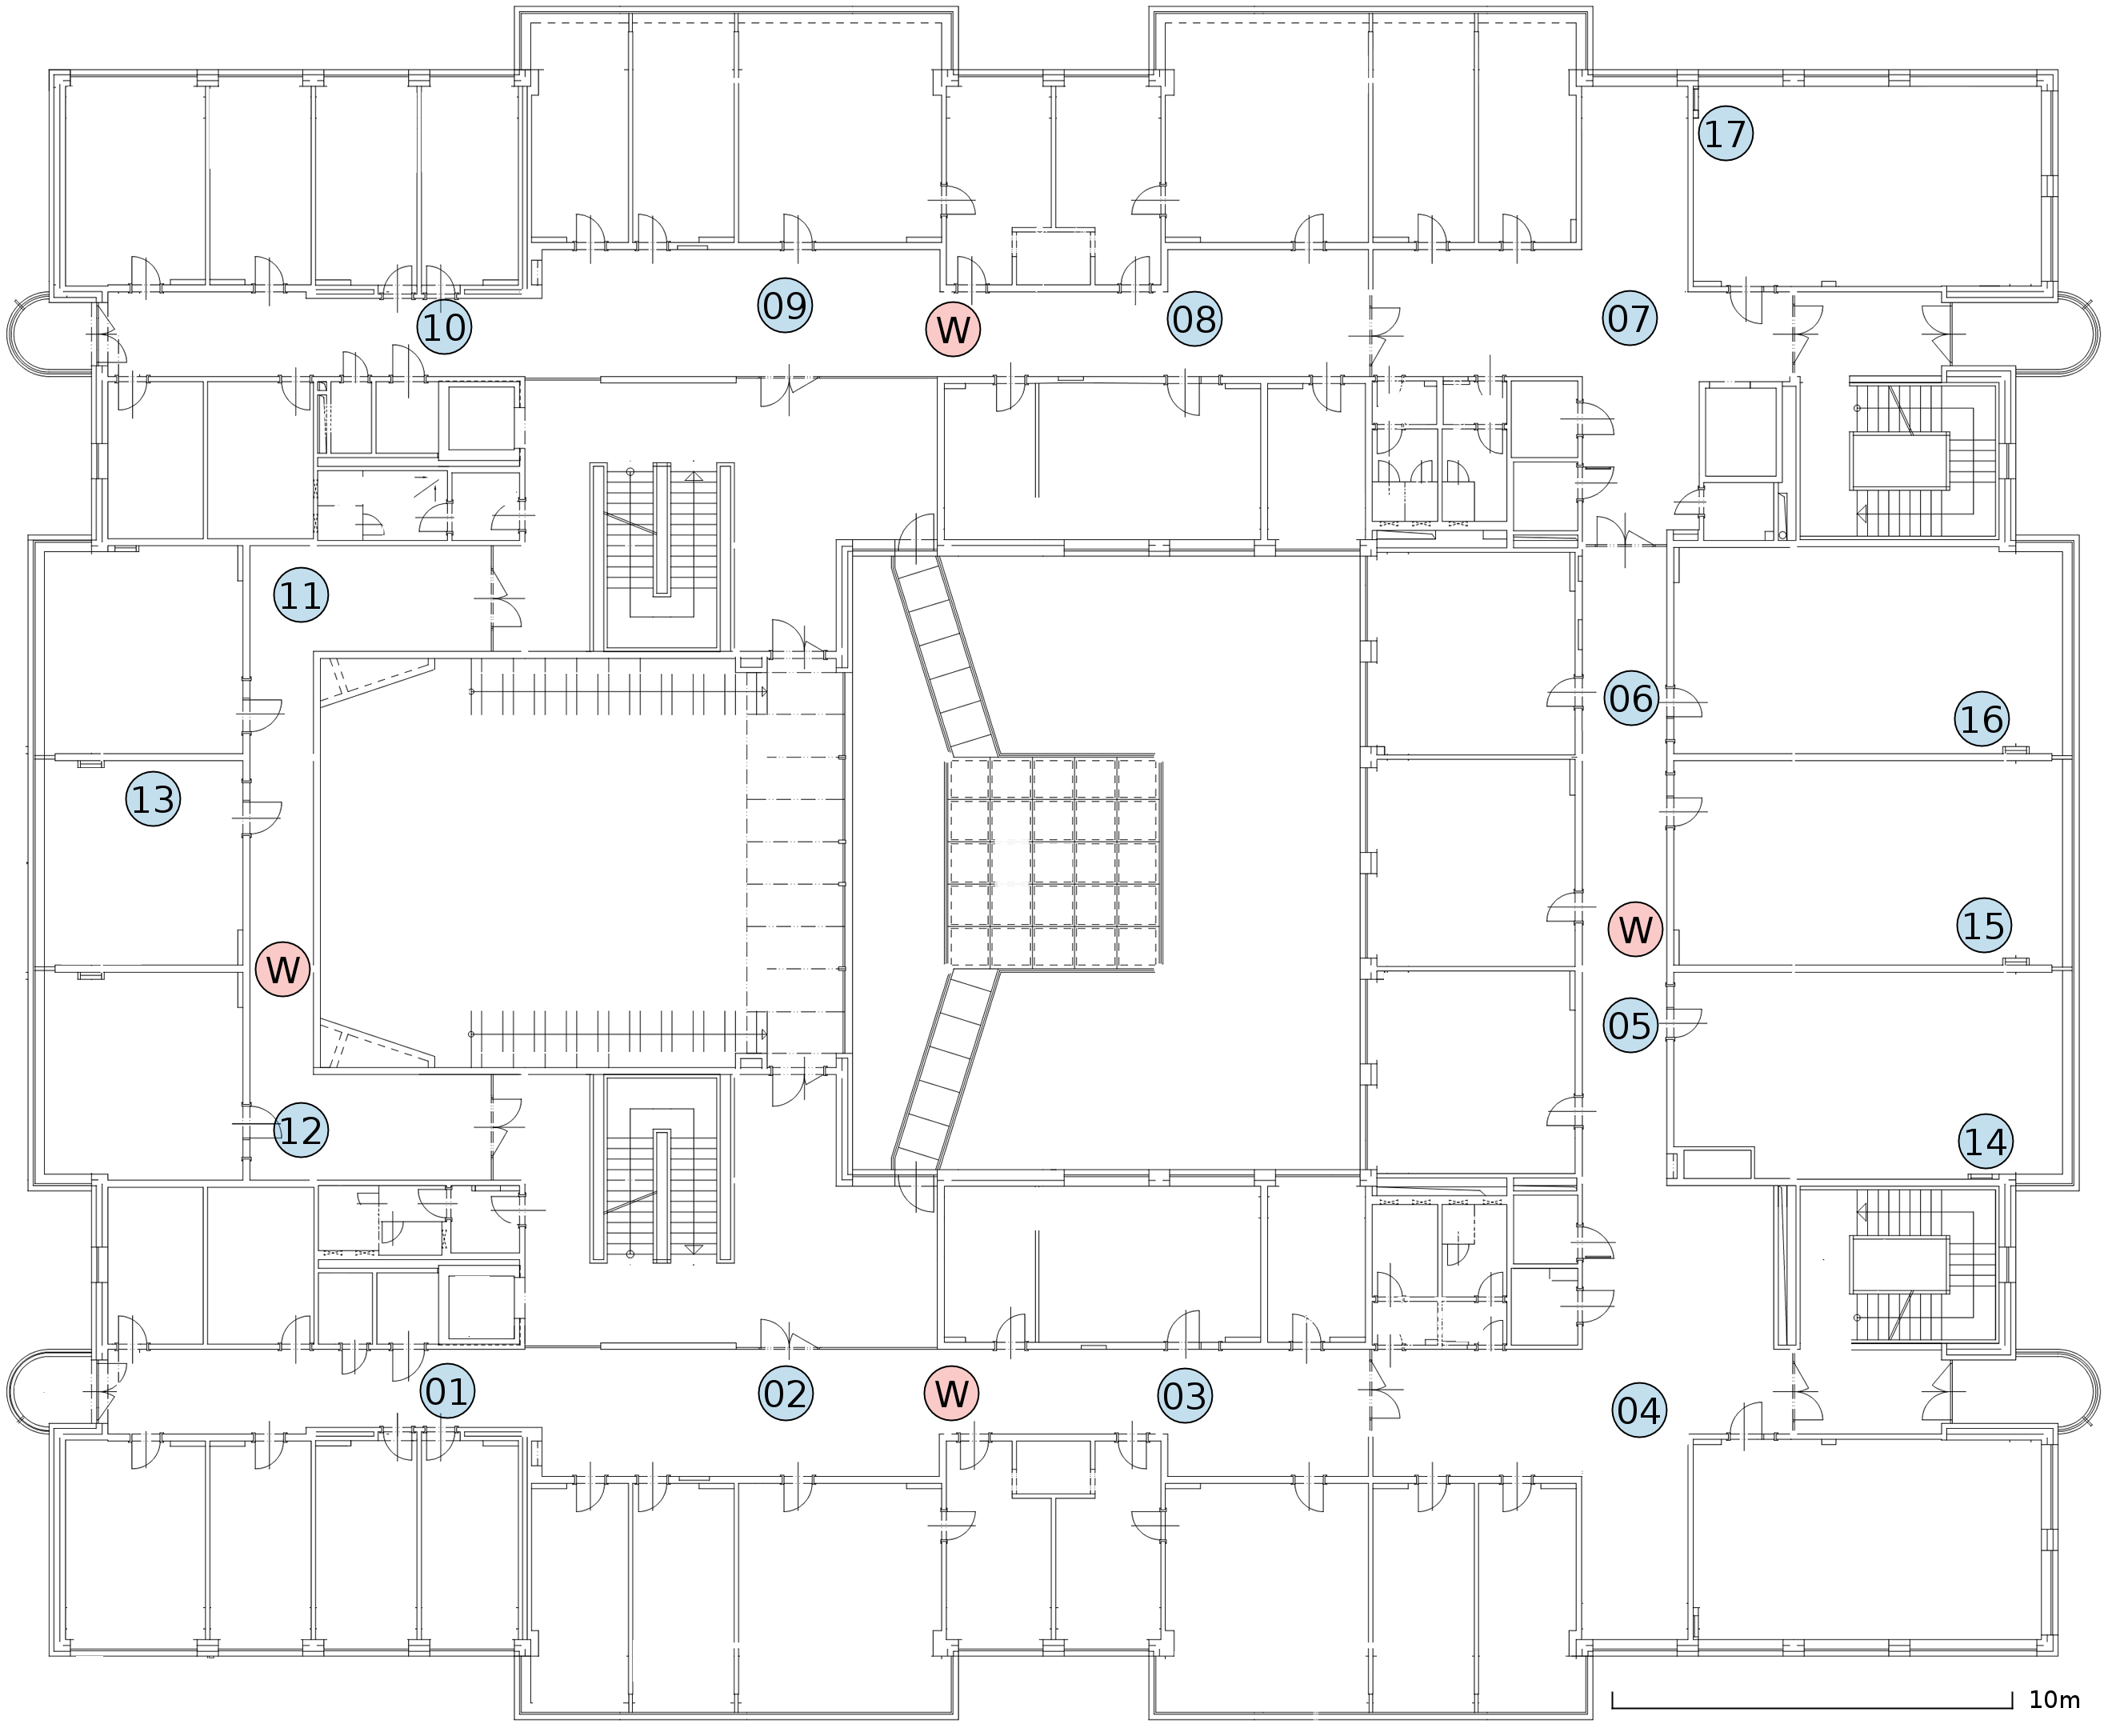
\includegraphics[width=0.8\textwidth]{img/j3np}
		\par\end{centering}
	\caption{Map of deployed devices (based on \cite{IILUBLEB})}
	\label{fig01c06}
\end{figure}

\fref{fig01c06} shows environment and positions of deployed devices. There are four WiFi transmitters for \textbf{eduroam} network made by Cisco (marked as W) on this floor. They are permanently placed on the ceiling and their settings could not be altered. Each marked place has usually more than one of them, typically at least two to enable broadcasting in 2.4 GHz and 5 GHz band. Their TX and power is automatically adjusted to help mitigate interference and signal coverage problems.

The other devices marked by numbers from 1 to 17 are Bluetooth Low Energy beacons placed evenly in the corridors and classrooms on the floor. Their broadcast parameters were set to advertising interval of 100 ms and the TX power of 0 dBm. Corridor beacons are placed in positions about 10 meters apart from others \cite{IILUBLEB}. Since the beacons were placed two years ago there was a possibility of battery depletion and malfunction. After multiple tests it was confirmed that two beacons had their battery depleted (1, 4), one was reconfigured (14) and one was misplaced and had to be changed (5).

\section{Evaluation approach}\label{sec:EvaluationApproach}
Basic approach for evaluation is the same as in previous years, using solution created by Pavel Kriz in \cite{IILUBLEB}. This approach is based on WKNN algorithm used to compare fingerprints against each other by selecting one and calculating its position using other fingerprints. Basic premise of this evaluation is to pick one fingerprint, forget its position and try to calculate it via specific amount of closest neighbors. This calculated value is then compared to the real one and difference between these values is the localization error in meters. Advantage of this approach is that it can be done in only one phase instead of two, since online phase is supplemented by one selected fingerprint. Second advantage is an easy implementation and calculation of error difference because both calculated and real positions are known.

This evaluation is implemented to be used only for one fingerprint and compare it to the others. It evaluates BLE and WiFi signals separate or together so it can provide an insight on which technology is better and if combining them improves the precision. This evaluation program also enables filtering out data not used for analysis, which are records of devices other than mentioned BLE beacons and WiFi access-points. It is developed to not differentiate between technologies of recording devices and it had to be expanded to support this feature. Few following implementations were added to this evaluation approach.

\begin{itemize}
	\item Filtering data by the device type, which is an important part to enable testing only for a specific device type. These fingerprints are tested only against its own technology and results can be used to compare precisions between different technologies.
	\item Selecting fingerprint group, it selects multiple fingerprints to be tested at the same time. This selection is done using scan id information, meaning both scan originated at the same time and place on different devices. Both fingerprints are then tested individually but the results are combined together with the aim to improve overall localization accuracy. This approach has two testing types, first is running the test against fingerprint's own technology and the other against all of them.
	\item Combining data from multiple fingerprints based on device technologies and consider it as one. Fingerprints are selected based on their scan id and all scanned data are cloned into mobile fingerprint combining them together. It can copy data only from selected radio technologies or all of them to provide the best overall localization.
\end{itemize}

All of these different approaches will enable to compare technologies and to assess which approach has the lowest localization error so it could be used in the future. 

\subsection{WKNN}\label{sec:WKNN}
This approach is an extension of algorithm \textbf{K-Nearest Neighbors} (KNN) with \textbf{Weights} making it \textbf{WKNN}. KNN is based on the idea that unclassified individual should belong to the same class as its nearest neighbor in the data set \cite{HGAfC}. It calculates the position based on the locations of selected K-nearest neighbors, where K change influences the accuracy of this algorithm. Extended with weights, WKNN can make some neighbors or data more valuable than other ones. In this case, closer fingerprints have higher weight and will be used to calculate position by Euclidean distance formula. The equation for fingerprint $f = (f_1,f_2,...,f_n)$ from the $i$th fingerprint $S_i = (s_{i1} ,s_{i2},...,s_{in})$ can be expressed by following formula \cite{IILUBLEB, HGAfC}:

$$D_i = \sqrt{\strut\sum_{j=1}^{N}(f_j-f_{ij})^2}\ ,$$

where N is a number of unique transmitters in the measurement.

These distance values are sorted and based on them, first $k$ fingerprints are chosen to calculate weighted estimate of position $P$ of measured fingerprint. It can be achieved by using their known positions $P_i[x_i,y_i]$ in a following formula:

$$ P = 
\frac
	{\strut\sum_{i=1}^{k} P_i Q_i}
	{\strut\sum_{i=1}^{k} Q_i},\
where\
	Q_i = \frac{\strut 1}{\strut D_i}.$$

WKNN algorithm was chosen because it is easy to implement and result data are not difficult to interpret.

\section{Data collection}\label{sec:DataCollection}
Data was collected at 105 evenly-spaced (2m) positions of single floor of Campus building. Each position was measured four times, in two different headings (north, south) and with two device orientations to prevent signal obstruction. Using both devices, 105 positions and 4 scans per position resulted in 840 different measurements, consisting of 466 411 BLE and 73 757 WiFi individual RSSI samples making it 540 168 in total.

Each of the scans was run for 30 seconds on both devices at the same time to provide equal environment. It is not really feasible to run such a long scan in one run, so the decision was made to split it into sub-scans with smaller time intervals. BLE beacons have advertising interval set to 100 ms and scanner length could be set to this number but it is set to 200 ms to prevent packet loss between the scans. Localization using WiFi usually does not need a big amount of data to provide good precision, thus scanner is set to run every 5 seconds. One problem with this scanner is that Android does not allow to set scan length or cancel running WiFi scan, only thing that can be canceled is listening for new WiFi records but scan could still be running in the background. Due to this limitation it can happen that current scan receives data from previous one, this is not prevented in the application but such data can be filtered out during evaluation by their scan time, which is usually set to 0. Cellular and sensor scanner are set to the same length as WiFi since this data is used only as complimentary information and it also helps to reduce fingerprint data size.

Three data collections were run during application development and data from the last one were used for evaluation. To consider fingerprint viable it must contain at least 20 records for Bluetooth Low Energy and WiFi, otherwise it needs to be deleted and re-scanned.

\subsection{First data collection}\label{sec:FirstDataCollection}
This first collection was meant as a test run in real environment and it consisted of scanning ten spots, each was scanned three times for 20 seconds to check if the scanner is reliable. It revealed two main problems with the current scanner implementation.

First, WiFi scanner on wear device was not able to record any data. It was highly likely that there was a problem with the scanner and also scan length, since quick 30 seconds test showed data added at the last second. This was fixed by two main changes, increasing scan length to 30 seconds and more importantly wear device now starts a \enquote{dummy} WiFi scan right after the application is displayed, just before an actual scanning is triggered. These changes helped to improve this scanner and it does not create any problems since there is little time span between this \enquote{dummy} scan and the actual scan, usual time difference is in milliseconds. This issue was also recorded only when wear was not connected to any WiFi network.

Second, not enough data was received by BLE scanner, usually less than by WiFi scanning. Data from previous years showed that each scan usually has hundreds of BLE records but this scanner was able to only collect around 50 of them. It was later discovered that sub-scan times were not properly set for AltBeacon library and scanner was run for 1 second instead of 200 milliseconds with only one device record per scan.

After both of these issues were fixed, second data collection was done to collect the data for evaluation. Final thing figured out during this collection is that wear device was not able to record any Cellular information even though specification shows it should support LTE technology, but that was probably because there were no LTE towers in range. 

\subsection{Second data collection}\label{sec:SecondDataCollection}
This collection was meant to be the final one and the data were supposed to be used for evaluation, but there were few more problems revealed after all data was collected. Data seemed fine at the first look but evaluation showed problems in BLE precision compared to the results from previous years. For a start, data analysis resulted with around 30 fingerprints removed from the testing due to no floor BLE beacons found and most of these fingerprints originated on wear device.

\vspace*{6pt}
\begin{table}[h]
	\begin{center}
		\begin{tabular}{ l C{2cm} C{2cm} C{2cm} }
			\hline
			Max error (m) & BLE & WiFi & Combined \\ 
			\hline
			All devices & 27 & 14 & 11 \\ 
			Mobile & 30 & 14 & 11 \\ 
			Wear & 31 & 11 & 11 \\ 
			\hline
		\end{tabular}
		\caption{Maximum errors for second data collection}
		\label{tab01c06}
	\end{center}
\end{table} 
\vspace*{-\baselineskip}
\vspace*{6pt}

\tref{tab01c06} shows a summary of maximum errors in meters for collected data, it shows that BLE errors can be two or three times higher than those of WiFi, reaching over 30 meters error which would place the device on the other side of the building. Mean and median errors showed the same trend, so next step was to test if some beacons are missing in the data and display all fingerprint errors on the map to find the worst locations.

\begin{figure}[H]
	\begin{centering}
		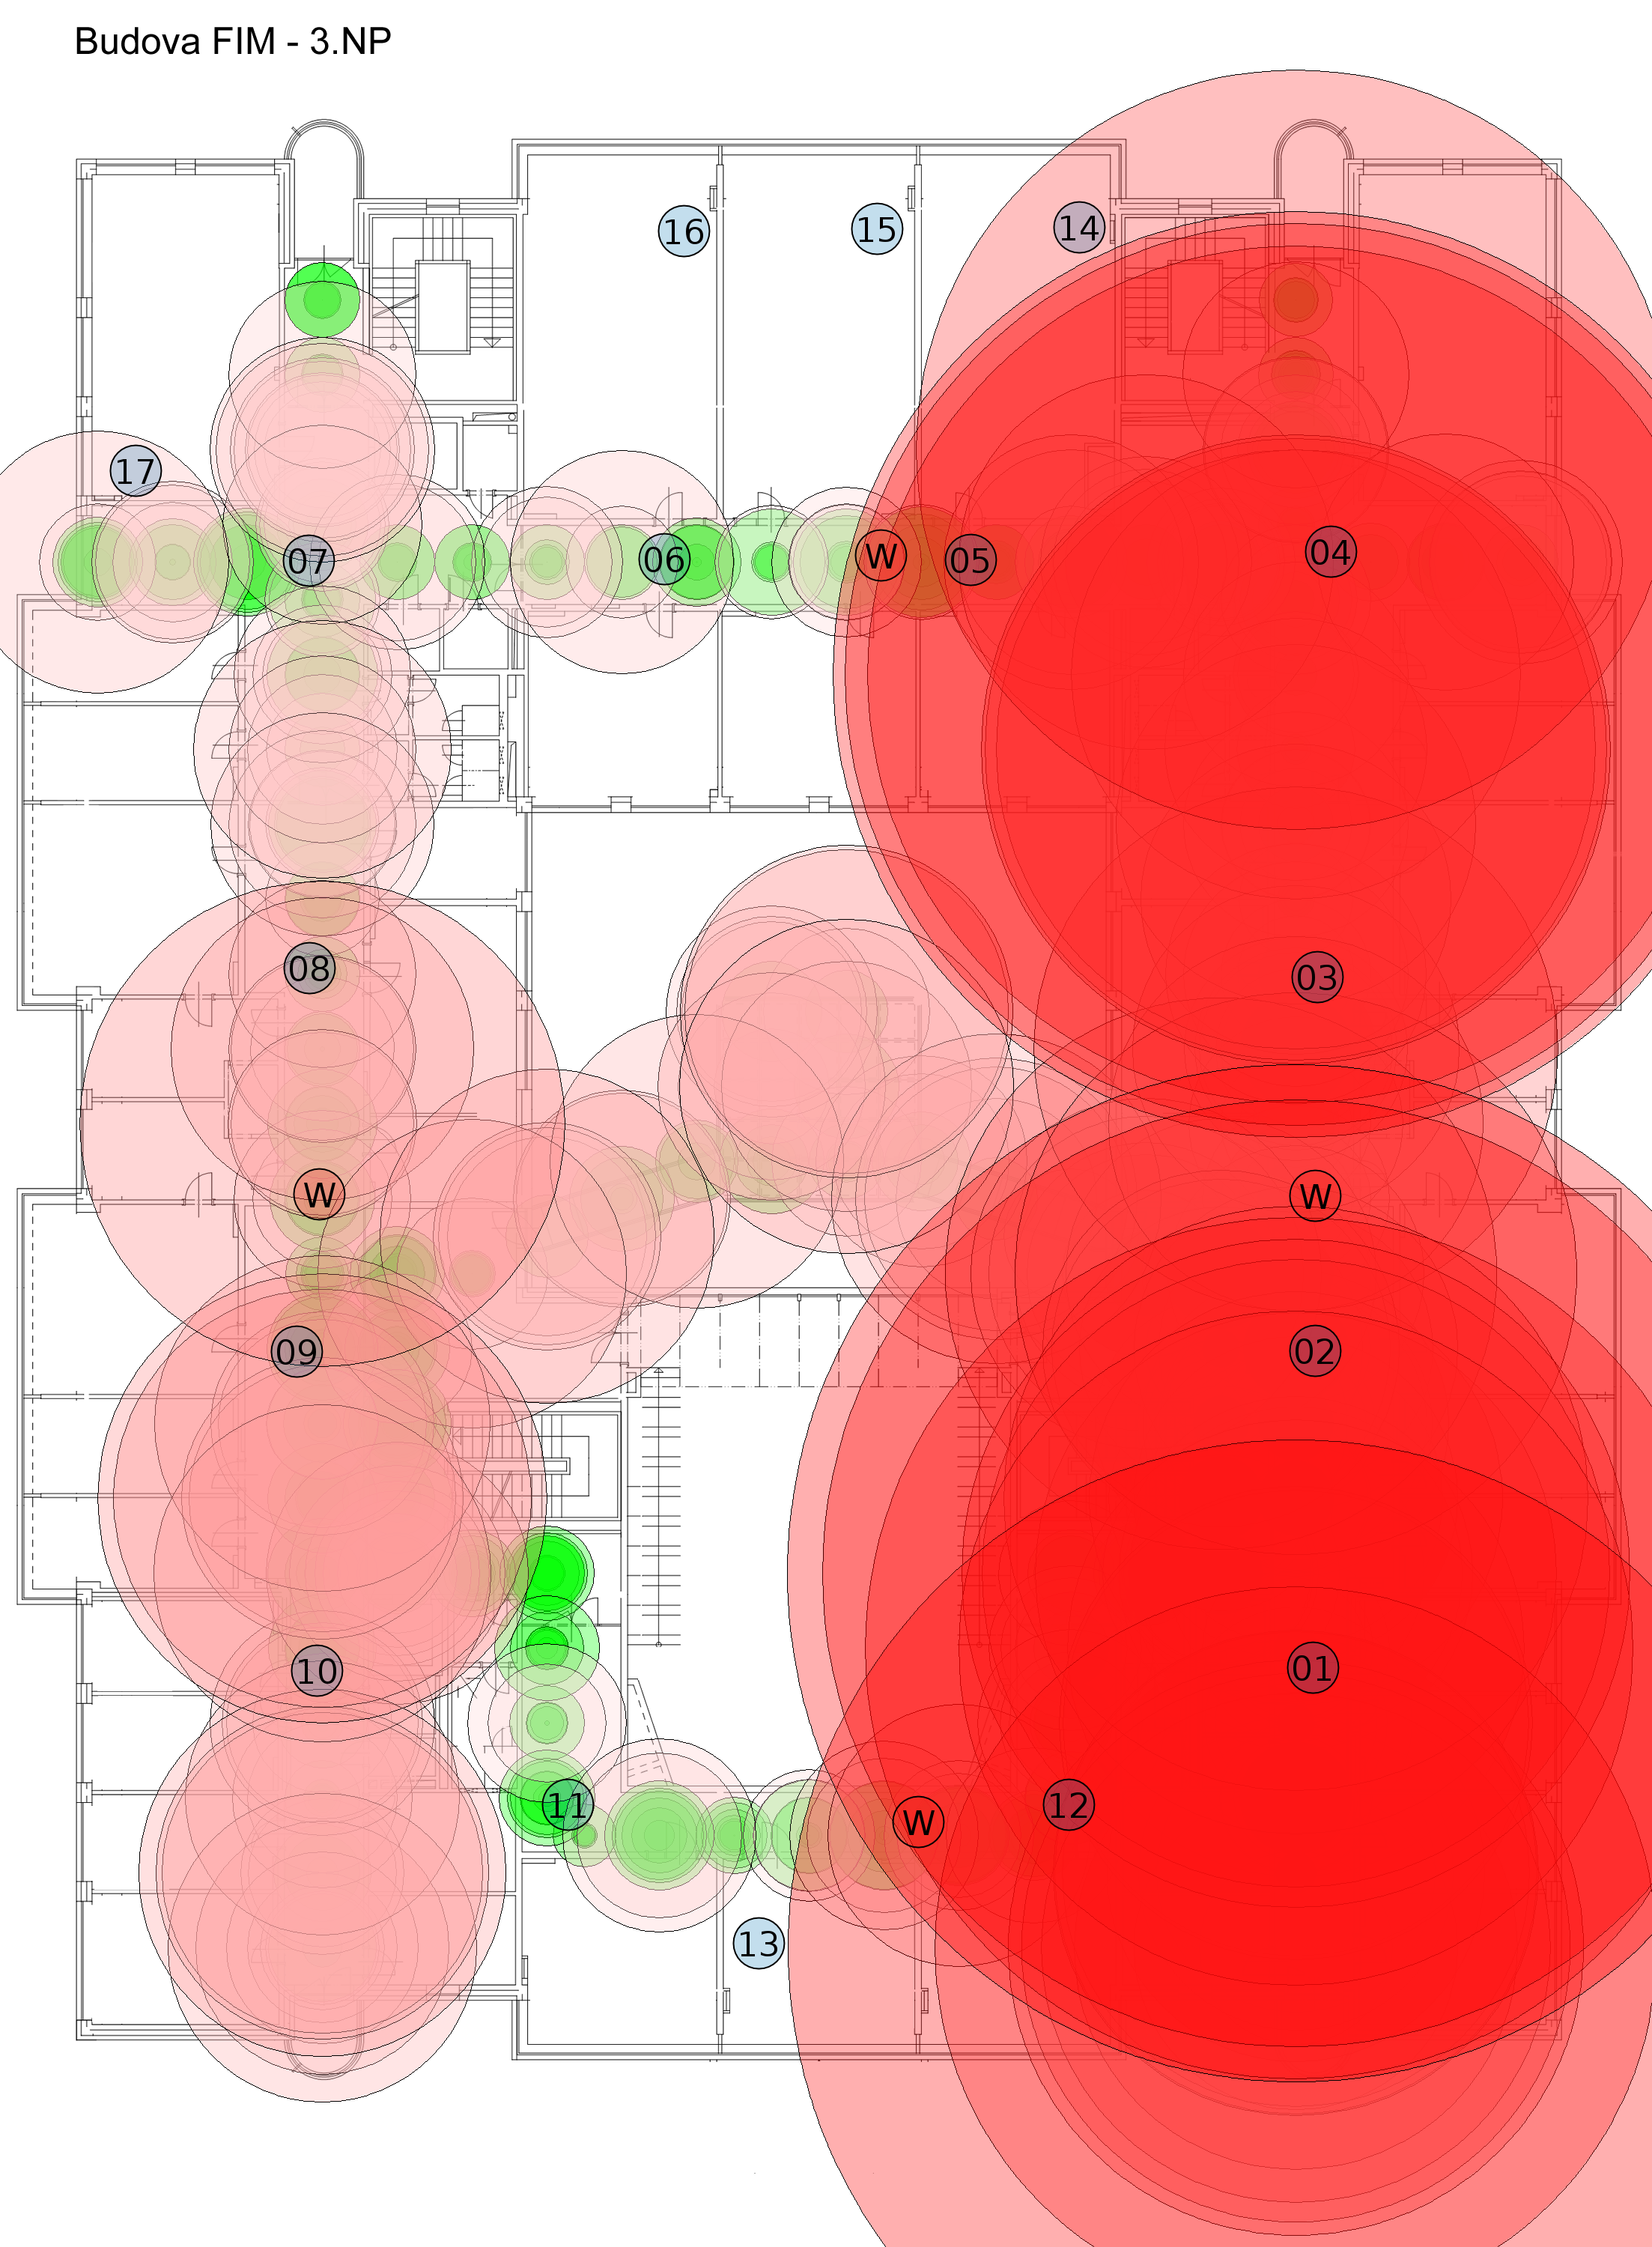
\includegraphics[width=0.4\textwidth]{img/second_data_collection_errors}
		\par\end{centering}
	\caption{Map of errors for BLE in meters for all fingerprints}
	\label{fig02c06}
\end{figure}

\fref{fig02c06} shows errors for BLE scanning on the map with two indications of error value. First, circle size is calculated from error number, higher errors are displayed using bigger circles. Second, fingerprints with error under three meters have green color and those above have color based on their error in the red spectrum, higher error results in more saturated red. Judging based on these information, evaluation seems to be the worst near beacons 1 and 4, which were later found out to be out of power. Next evaluation using differences in advertising interval revealed beacon number 14 reconfigured to different settings. And final tests, by visual checks if all beacons are in place, confirmed that beacon number 5 was moved and had to be replaced. All of these tests resulted in four malfunctioning beacons all over the floor and deeming the data not viable for further evaluation, hence a new round of data collection was required.

Since this was a complete data collection it also served as a test for wear device and how long it can stay operational while scanning. Multiple data was collected to measure this, such as start and end time, number of places and fingerprints scanned and of course power status. Wear device is never used under 15\% because this is the threshold when power saving is turned on and device shuts down all non-essential functions.

\begin{table}[h]
	\begin{center}
		\begin{tabular}{ l C{2cm} C{2cm} C{2cm} C{2cm} }
			\cline{2-3}
			& \multicolumn{2}{c}{\% Battery power} & & \\
			\hline
			Time & Start & End & Places & Fingerprints \\ 
			\hline			
			2:50 & 100\% & 15\% & 30 & 240 \\
			2:40 & 100\% & 17\% & 37 & 296 \\
			1:55 & 100\% & 35\% & 12 & 96 \\
			1:20 & 100\% & 70\% & 18 & 144 \\
			0:45 & 30\%	& 15\% & 8 & 64 \\
			\hline
		\end{tabular}
		\caption{Scanning information for wear (second scan)}
		\label{tab02c06}
	\end{center}
\end{table}

\tref{tab02c06} shows a summary of all important information for wear scanning evaluation. First, comparing the percentages of power with time shows that wear device cannot usually last for more than three hours of scanning, which is no enough, since all the scans together took about 8 hours to complete. The two longest scans show that wear can scan for around 35 places without the need to re-charge, which is confirmed by the shortest scan where scanning 8 places takes around 45 minutes and 15\% of the device battery. There are also some exceptions, for instance, the third scan which was done in the middle of Campus building where there are no beacons and it was needed to re-scan multiple places many times to achieve set requirements for fingerprints mentioned in previous chapter.

\subsection{Third data collection}\label{sec:ThirdDataCollection}
Third and final data collection was conducted after all beacons were checked and fixed. Scanning showed only one single problem and that was again with the WiFi scanning on the wear, where no records were found after around 10 spots (80 fingerprints) collected. This was not a huge issue because it has two easy fixes. First, restarting the device which will enable to scan for 10 more spots without problems. Second, turn off and on the WiFi receiver on the wear device but this fix only works for next two or three scans, so it is not ideal. Both of these solutions were used based on the situation but both devices were always turned on and off after 15 successfully scanned spots.

\begin{table}[h]
	\begin{center}
		\begin{tabular}{ l C{2cm} C{2cm} C{2cm} C{2cm} }
			\cline{2-3}
			& \multicolumn{2}{c}{\% Battery power} & & \\
			\hline
			Time & Start & End & Places & Fingerprints \\ 
			\hline			
			2:40 & 100\% & 15\% & 37 & 296 \\
			2:00 & 100\% & 33\% & 30 & 240 \\
			1:10 & 100\% & 58\% & 18 & 144 \\
			0:45 & 50\% & 22\% & 11 & 88 \\
			0:40 & 40\% & 15\% & 9 & 72 \\
			\hline
		\end{tabular}
		\caption{Scanning information for wear (third scan)}
		\label{tab03c06}
	\end{center}
\end{table}

For this scan, only one specific change was made and that was starting a \enquote{dummy} scan on a mobile device. Before this collection it was implemented only on wear device, which was changed to ensure that scanning code for both devices is completely the same and thus provide equal environment. Collecting of all fingerprints took about 7 hours and 15 minutes, in this case, which is almost an hour less than the length of previous scanning which took 8 hours and 10 minutes. Battery information in \tref{tab03c06} confirms the results from previous scanning and shows that wear device cannot scan more than three hours at the time before reaching power saving mode threshold. This feature can now be disabled after the new update of wear device system but it was not used since there is no guarantee it will disable all parts of power saving and provide equal environment.

\begin{figure}[h!]
	\begin{centering}
		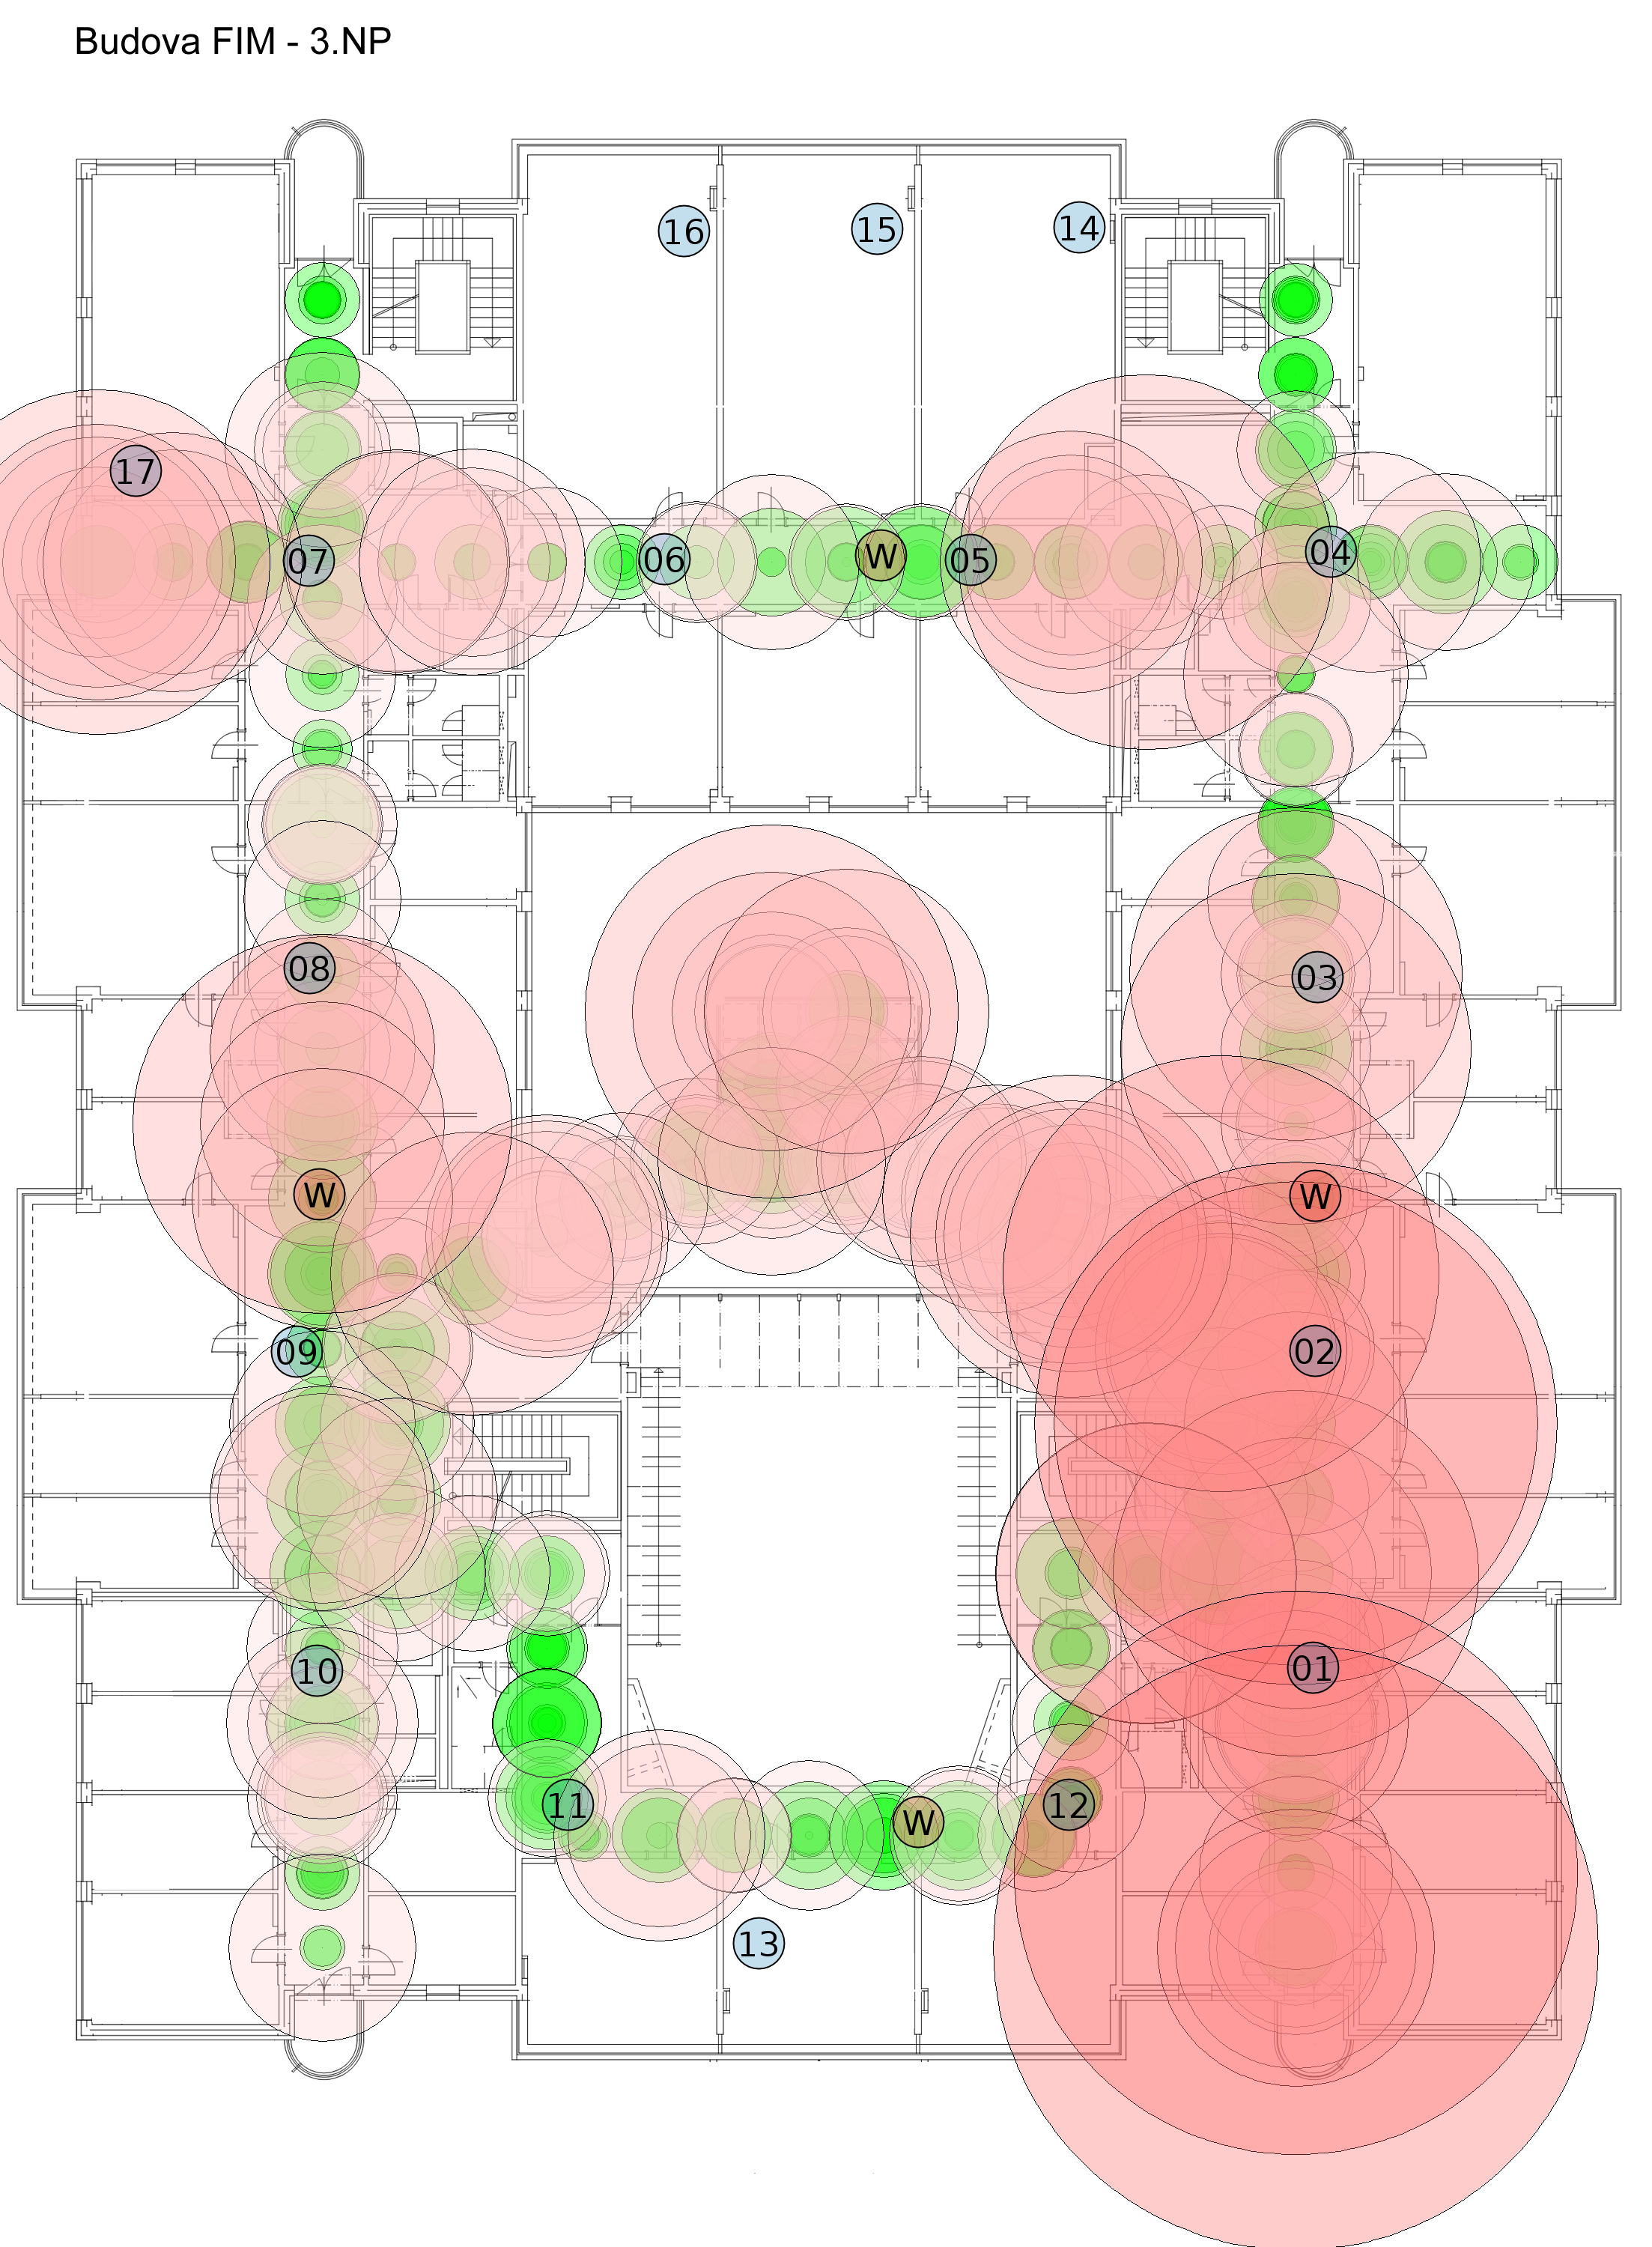
\includegraphics[width=0.4\textwidth]{img/third_data_collection_ble_errors}
		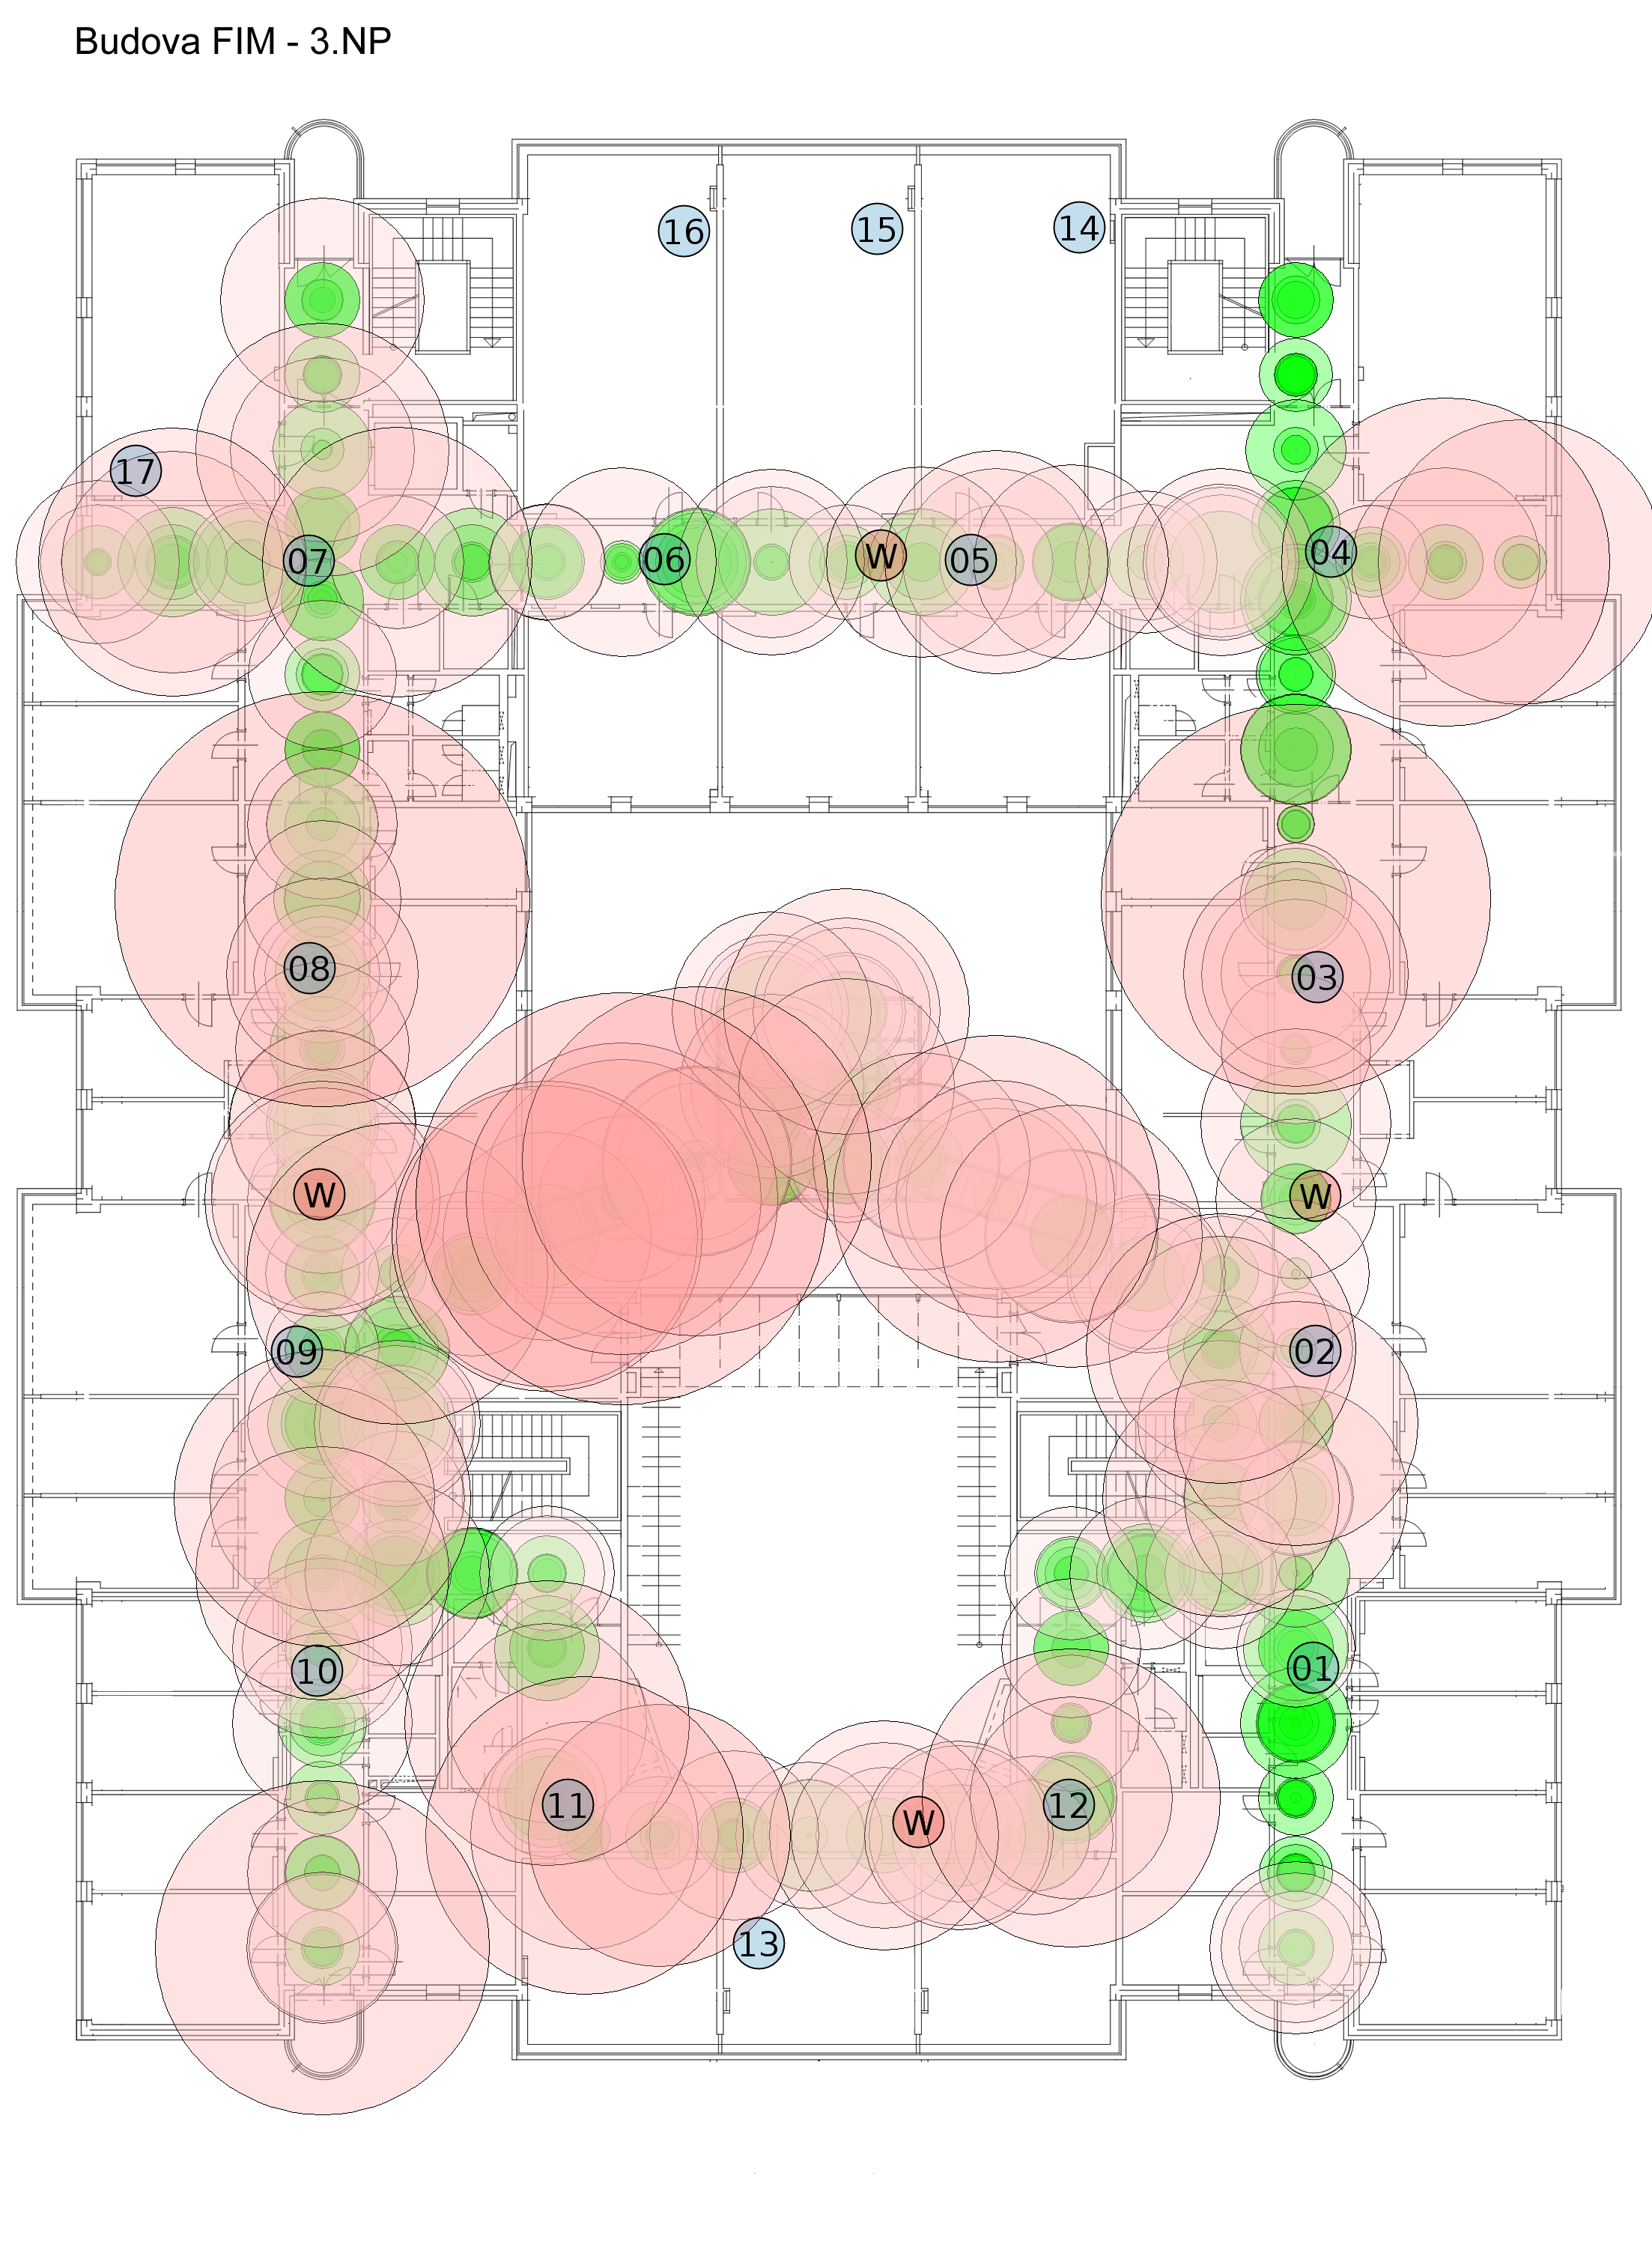
\includegraphics[width=0.4\textwidth]{img/third_data_collection_wifi_errors}
		\par\end{centering}
	\caption{Map of errors for BLE (left) and WiFi (right)}
	\label{fig03c06}
\end{figure}

\fref{fig03c06} shows two images, one per radio technology, of all fingerprint errors on the map, creating eight overlapping circles on each spot. WiFi seems more precise in comparison with BLE and there might still be some issues around beacon 1. Places with one or two light red circles will usually be improved by other fingerprints on that spot but the others could increase overall localization error. On the other hand, comparison of this figure and \fref{fig02c06} shows a decrease of BLE errors for this scanning. Looking at the differences between WiFi and BLE suggests that WiFi should have less errors and better accuracy but there might be issues for both technologies in the middle of the building.

\section{Evaluation}\label{sec:Evaluation}
Evaluating of all the data has multiple approaches and combinations since in needs to consider information, such as algorithm implemented, multiple device types and radio signal technologies. During the second data collection it was figured out that wear device is not able to scan for Cellular records so these radio signals will not be tested in the evaluation. First thing that needs to be decided is which $k$ value to use in following evaluations using WKNN algorithm and after that multiple tests can be run to compare device types and how fingerprints can be used to improve each other.

\subsection{Decide K values for WKNN}\label{sec:TestingKValuesForWKNN}
To select proper $k$ value all data was tested without their device information, thus putting all of them together and test them against each other. Only $k \in \{2, 3, 4\}$ were used in the selection process because using $k = 1$ defeats the purpose of WKNN algorithm and setting $k > 4$ results with too big errors. Following table shows a summary of mean, median and maximum errors in meters for all tested $k$ values.

\vspace*{6pt}
\begin{table}[h]
	\begin{center}
		\resizebox{\textwidth}{!}{
			\begin{tabular}{ l C{2cm} C{2cm} C{2cm} | C{2cm} C{2cm} C{2cm} | C{2cm} C{2cm} C{2cm} }
				\cline{2-10}
				& \multicolumn{3}{c|}{K = 2} & \multicolumn{3}{c|}{K = 3} & \multicolumn{3}{c}{K = 4} \\
				\hline
				& BLE & WiFi & Combined & BLE & WiFi & Combined & BLE & WiFi & Combined \\ 
				\hline	
				Mean & 2.25 & 1.77 & 1.52 & 2.20 & 1.76 & 1.52 & 2.15 & 1.80 & 1.56 \\
				Median & 1.93 & 1.06 & 1.02 & 1.76 & 1.30 & 1.22 & 1.61 & 1.32 & 1.06 \\
				Maximum & 12.90 & 11.11 & 10 & 12.59 & 11.38 & 9.67 & 13.28 & 10.60 & 9.39 \\
				\hline
			\end{tabular}
		}
		\caption{List of errors for multiple K values}
		\label{tab04c06}
	\end{center}
\end{table}
\vspace*{-\baselineskip}
\vspace*{6pt}

Mean and median information are the main factors used to decide which $k$ to use and maximum is meant only as a complimentary information. Considering values by technology it seems $k = 2$ is best for WiFi and $k = 4$ for BLE so it will be decided between these two. Combining technologies together shows better mean and median for $k = 2$ and maximum for $k = 4$ and because main values are better when using $k = 2$ it was selected for following evaluations. It also achieves better accuracy with WiFi, which is more precise than BLE technology, and this value was also already tested and used in previous years \cite{IILUBLEB}.

\begin{figure}[h!]
	\begin{centering}
		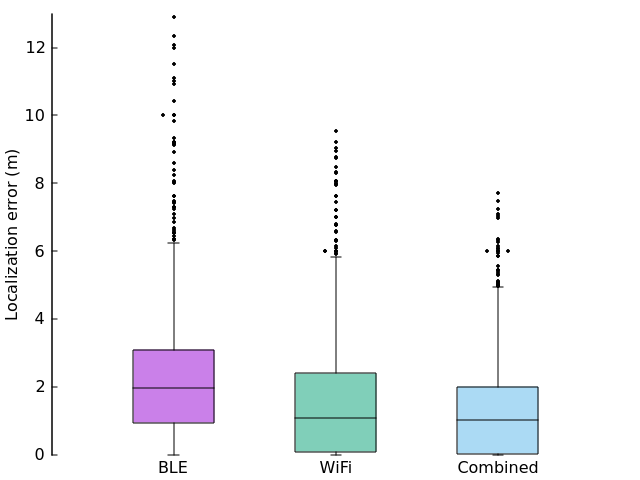
\includegraphics[width=0.5\textwidth]{img/wknn_errors_classic}
		\par\end{centering}
	\caption{Comparison of localization accuracy for $k = 2$}
	\label{fig04c06}
\end{figure}

\fref{fig04c06} shows comparison for both radio technologies used for evaluation and their combinations. It correlates with \tref{tab04c06} showing WiFi as a better technology and their combination improved over using only single one of these two technologies. This graph is also used to compare this evaluation method with future iteration of WKNN algorithm which consider technology of recording device when evaluating fingerprints.  

\subsection{Compare device technologies}\label{sec:CompareDeviceTechnologies}
After it is known which parameters to use, evaluation of the device technologies can be started. For this part minimum of data filtering was used and all the fingerprints were tested based on their device technology. To compare overall precision all data were also put together and tested against each other without taking device technology into consideration, meaning position of mobile fingerprints could be calculated using wear fingerprints and vice versa. This is not the best approach since it defeats the purpose of using different device types but it is easily implemented for the first round of evaluation.

\vspace*{6pt}
\begin{table}[h]
	\begin{center}
		\resizebox{\textwidth}{!}{
			\begin{tabular}{ l C{2cm} C{2cm} C{2cm} | C{2cm} C{2cm} C{2cm} | C{2cm} C{2cm} C{2cm} }
				\cline{2-10}
				& \multicolumn{3}{c|}{Mean error (m)} & \multicolumn{3}{c|}{Median error (m)} & \multicolumn{3}{c}{Max error (m)} \\
				\hline
				& BLE & WiFi & Combined & BLE & WiFi & Combined & BLE & WiFi & Combined \\ 
				\hline	
				Wear & 2.27 & 2.67 & 2.21 & 2.00 & 2.10 & 2.00 & 12.90 & 11.11 & 10 \\		
				Mobile & 2.05 & 0.88 & 0.85 & 1.76 & 0.80 & 0.88 & 11.50 & 8 & 6.06 \\
				All devices & 2.25 & 1.77 & 1.52 & 1.93 & 1.06 & 1.02 & 12.90 & 11.11 & 10 \\
				\hline
			\end{tabular}
		}
		\caption{Device comparison: mean and max errors (in meters)}
		\label{tab05c06}
	\end{center}
\end{table}
\vspace*{-\baselineskip}
\vspace*{6pt}

\tref{tab05c06} shows the comparison of device fingerprints and their calculated mean and max error values. BLE technology does not show much of a difference in devices, just about 0.2 meters which makes them comparable. The WiFi, on the other hand, shows a big difference between them and making mobile device a better solution with over two times lower mean error. Fingerprint data were checked to find precise reason behind this difference.

\begin{figure}[h!]
	\begin{centering}
		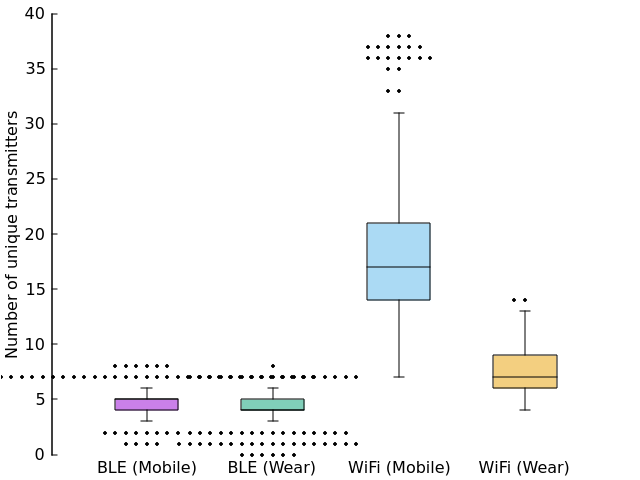
\includegraphics[width=0.6\textwidth]{img/number_of_transmitters}
		\par\end{centering}
	\caption{Number of transmitters for all fingerprints}
	\label{fig05c06}
\end{figure}

\fref{fig05c06} shows the number of transmitters for all fingerprints based on radio technology and device. It shows close numbers for BLE but there seems to be a lower amount of WiFi transmitters recorded by wear device. It seemed that wear was not able to record signals from some of them and after comparing the data from wear to mobile it was discovered that missing transmitters use 5 GHz technology. Mobile fingerprints contain over 7 300 WiFi records originating on access-points using 5 GHz and wear has 0 of them recorded, which means that wear device does not contain 5 GHz WiFi receiver. Records from 5 GHz are more precise than those of 2.4 GHz making this a reason why wear precision is not as good when comparing it to the mobile device. Every manufacturer is in control of hardware for its devices and Huawei decided not to implement it due to high power usage.

Combining data from both wireless technologies together and comparing devices shows wear error almost three times higher than the one of mobile device, thus increasing the error when combining all data together. It increases mean error from mobile only 0.85 to 1.52 combined and max from 6.06 to 10. Using only mobile device would result in better precision instead of combining them in this case. It is connected to already mentioned WiFi precision of wear device.

\begin{figure}[h!]
	\begin{centering}
		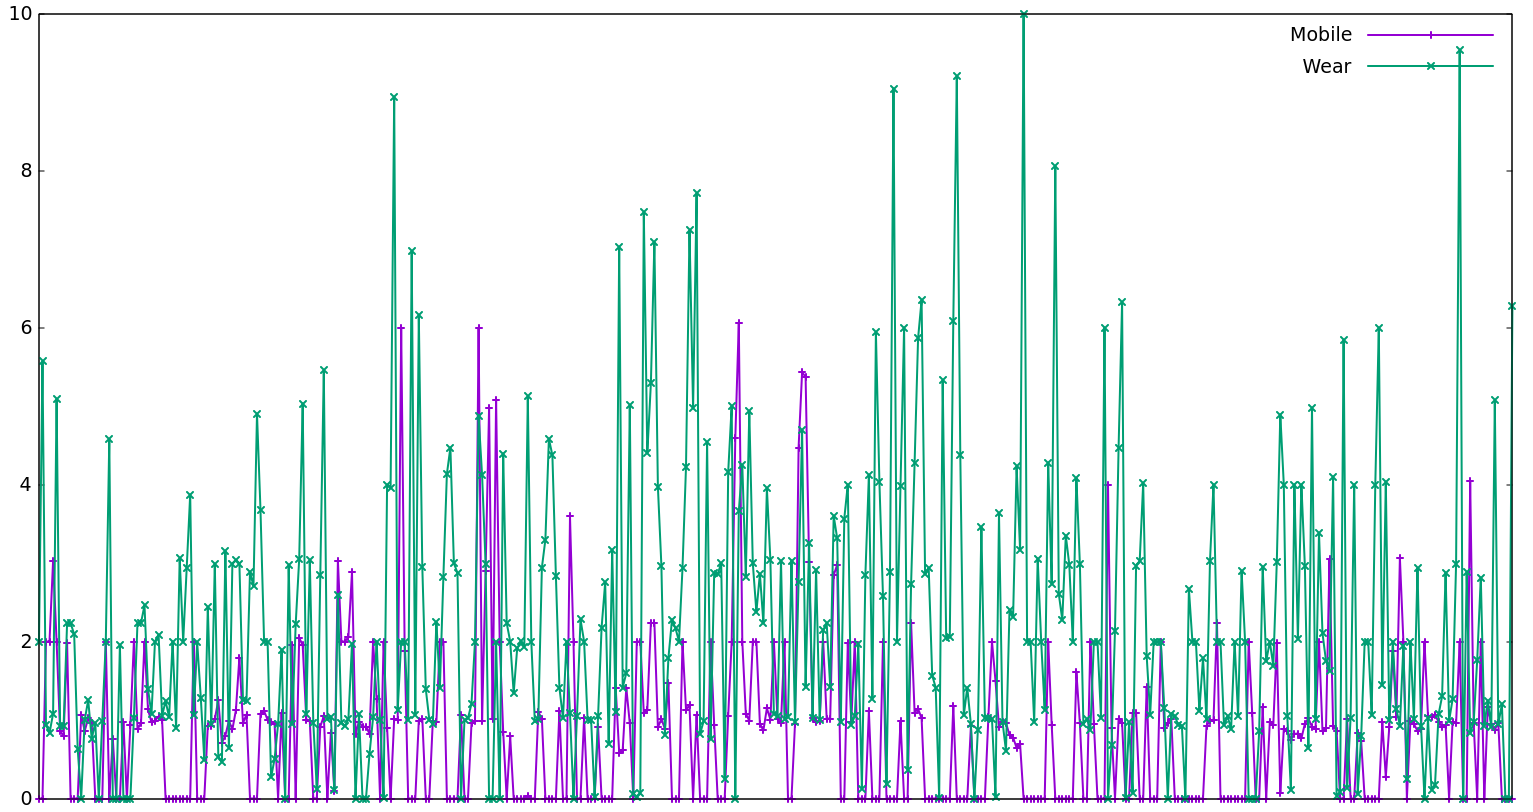
\includegraphics[width=0.95\textwidth]{img/wknn_errors_mobile_phone}
		\par\end{centering}
	\caption{Comparison of errors based on device}
	\label{fig06c06}
\end{figure}

To compare both technologies more precisely all fingerprint errors were sorted based on location and displayed in \fref{fig06c06}. This image confirms the information that using wear device fingerprints will result in higher error than mobile but there are few places where using wear is better, unfortunately not a lot of them. 

\subsection{Testing multiple fingerprints}\label{sec:TestingMultipleFingerprint}
Previous method is testing only single fingerprint against all other ones without the device type information. Improving upon previous design this evaluation selects multiple, two in this case, fingerprints with different origin device and runs the WKNN algorithm on them. These fingerprints have to be from the same location and also from the same scan group, which is identified by their scan id. All of these fingerprints have their location calculated and this information is then averaged to increase the location precision. This algorithm supports multiple technologies and it could be improved to support weights where specific technology, such as mobile, could have higher weight to reduce influence of technologies with worse precision.

There are two main implementations of this evaluation. First, calculates position for both fingerprints while ignoring  their device technology, each fingerprint location is calculated using all fingerprints, same as previous evaluation. Second, each of the fingerprint location is calculated only using its own device technology which is used to check the calculation influence based on the device, thus figuring out if testing fingerprints against their own technology can improve overall precision or make it worse.

\begin{table}[h]
	\begin{center}
		\resizebox{\textwidth}{!}{
			\begin{tabular}{ l C{2cm} C{2cm} C{2cm} | C{2cm} C{2cm} C{2cm} }
				\cline{2-7}
				& \multicolumn{3}{c|}{Compared to own technology} & \multicolumn{3}{c}{Compared to all} \\
				\hline
				& BLE & WiFi & Combined & BLE & WiFi & Combined \\ 
				\hline	
				Mean & 2.18 & 1.77 & 1.53 & 2.30 & 1.77 & 1.52 \\
				Median & 1.87 & 1.50 & 1.33 & 1.99 & 1.50 & 1.33 \\
				Maximum & 10.41 & 6.21 & 5.78 & 10.59 & 6.21 & 5.78 \\
				\hline
			\end{tabular}
		}
		\caption{List of errors for testing multiple fingerprints}
		\label{tab06c06}
	\end{center}
\end{table}

Comparing this \tref{tab06c06} with \tref{tab05c06} shows improvement in BLE precision but median values have gotten worse for WiFi making combined error higher from 1.02 to 1.33 meters compared to previous evaluation, which was expected. On the other hand there is a big decrease of maximum errors for both technologies decreasing combined error from 10 to 5.78 meters. From these values it is not easy to compare if precision got better or not but it can be used to compare if there is any influence of comparing fingerprints with its own technology. It shows slightly better values for BLE but those do not influence combined results which are almost completely the same, meaning there is no reason to compare fingerprint only with its own technology in this approach.

\begin{figure}[h!]
	\begin{centering}
		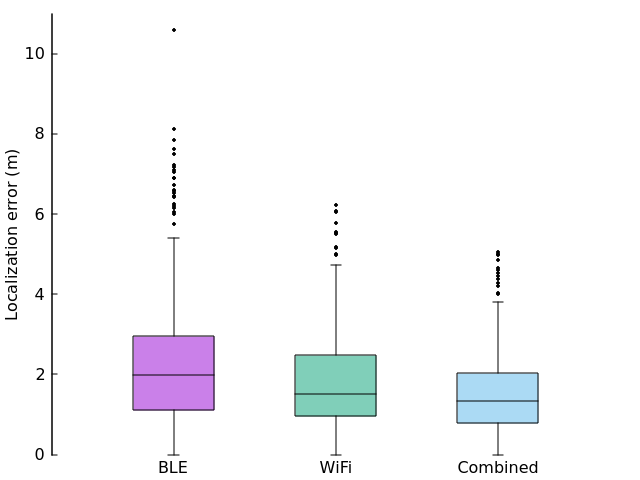
\includegraphics[width=0.5\textwidth]{img/wknn_errors_multiple}
		\par\end{centering}
	\caption{Comparison of localization accuracy for testing multiple fingerprints}
	\label{fig07c06}
\end{figure}

When comparing this figure with \fref{fig04c06} it shows a decrease of median accuracy mainly for WiFi which is also reflected on combined evaluation. Overall accuracy improves because errors are more clustered together and more evenly spread, which is confirmed by the decrease of maximum error from 10 to 5.78 making it more viable in complex environments and problematic places. This approach is not better then mobile only localization with these errors.

\subsection{Combining fingerprint data}\label{sec:CombiningFingerprintData}
Last evaluation did not prove tangible improvement of localization accuracy using wear technology in comparison with mobile only. For this reason next evaluation takes a different approach and combines data from multiple fingerprints, based on the device, into one. As it was already mentioned, fingerprints are grouped based on scan id, which identifies them as being taken at the same place and time using different devices. Data of such fingerprints are combined into single one, reducing their count for evaluation but hopefully increasing overall accuracy. Since there are multiple fingerprints combined together, the information about origin device is lost and there is no way to compare the technologies against each other.

There are two possible cases which were implemented for this evaluation. First, combine all data from a fingerprint group into single fingerprint. Second, combine only BLE data and keep WiFi from mobile, because it is known that wear WiFi precision is not sufficient and decreases the localization accuracy.

\vspace*{6pt}
\begin{table}[h]
	\begin{center}
		\resizebox{\textwidth}{!}{
			\begin{tabular}{ l C{2cm} C{2cm} C{2cm} | C{2cm} C{2cm} C{2cm} }
				\cline{2-7}
				& \multicolumn{3}{c|}{WiFi with BLE} & \multicolumn{3}{c}{BLE only} \\
				\hline
				& BLE & WiFi & Combined & BLE & WiFi & Combined \\ 
				\hline	
				Mean & 2.12 & 0.93 & 0.88 & 2.12 & 0.88 & 0.83 \\
				Median & 1.73 & 0.87 & 0.86 & 1.73 & 0.80 & 0.83 \\
				Maximum & 13.99 & 7.19 & 6.99 & 13.99 & 8.00 & 7.04 \\
				\hline
			\end{tabular}
		}
		\caption{List of errors for fingerprint combination}
		\label{tab07c06}
	\end{center}
\end{table}
\vspace*{-\baselineskip}
\vspace*{6pt}

This approach as a whole seems to be a big overall improvement in accuracy but with the increase of maximum error for BLE technology as a drawback. Copying all data together not only improves the precision, compared to previous evaluations, but also makes it comparable to using only mobile. In numbers from \tref{tab05c06}, mobile errors are 0.85m mean, 0.88m median and 6.06m maximum compared to 0.88m mean, 0.86m median and 6.99m maximum for this evaluation. Improvement is only in median but other two values increase in comparison. 

Second part of this approach, copying only BLE records to mobile fingerprints while keeping its current WiFi precision. With BLE error decreased this finally proved to be a better solution than using only mobile localization. Comparing the data from \tref{tab07c06} shows decrease of error for mean value from 0.85 to 0.83 meters which is around 2.4\% and median from 0.88 to 0.83 meters, reaching up to 6\% improvement over mobile only localization. One value that goes up is maximum error from 6.06 to 7.04 resulting in 16\% increase of this error.

\begin{figure}[h!]
	\begin{centering}
		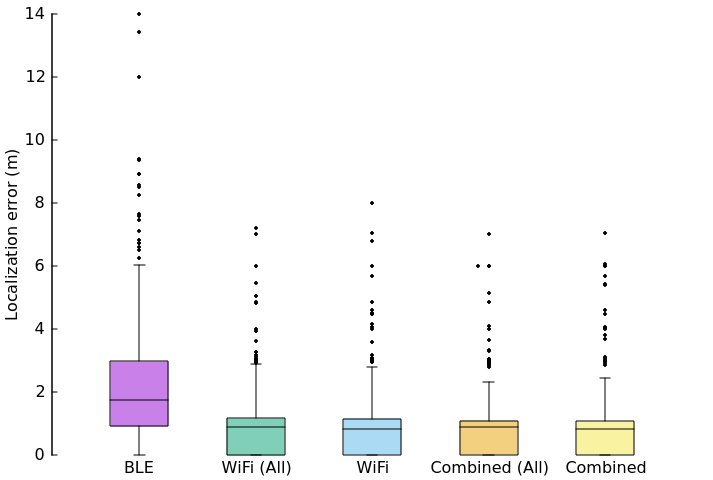
\includegraphics[width=0.6\textwidth]{img/wknn_errors_combined}
		\par\end{centering}
	\caption{Comparison of localization accuracy for combining fingerprints}
	\label{fig08c06}
\end{figure}

\fref{fig08c06} shows visualization of errors for both parts of this approach. BLE errors are the same for both cases and they seem to be somewhere between classic approach and testing of multiple fingerprints, since it has more clustered values compared to classic one but not as much as multiple fingerprints testing approach. However, WiFi shows the best localization precision compared to all previous iterations. Both of these approaches seems to be comparable and each one has a different merit to it. Combination of all data seems to increase mean and median but lowers the maximum errors, making it more reliable in problematic places, where the other approach seems to have the opposite result and being better overall.

\subsection{Map comparison}\label{sec:MapComparison}
To confirm previous results, all errors were displayed on the map to compare them and also to find problematic spots of the evaluation. These maps contain only combined errors of radio technologies to make it easier to read and not complicate it with differences between BLE and WiFi. There is also one other slight change to displayed data where errors under 200 centimeters are set to display as a circle with this precise error to make them more visible. This only influences last two images of \fref{fig09c06} because there are multiple positions with 0 meters error fingerprints.

\begin{figure}[h!]
	\begin{centering}
		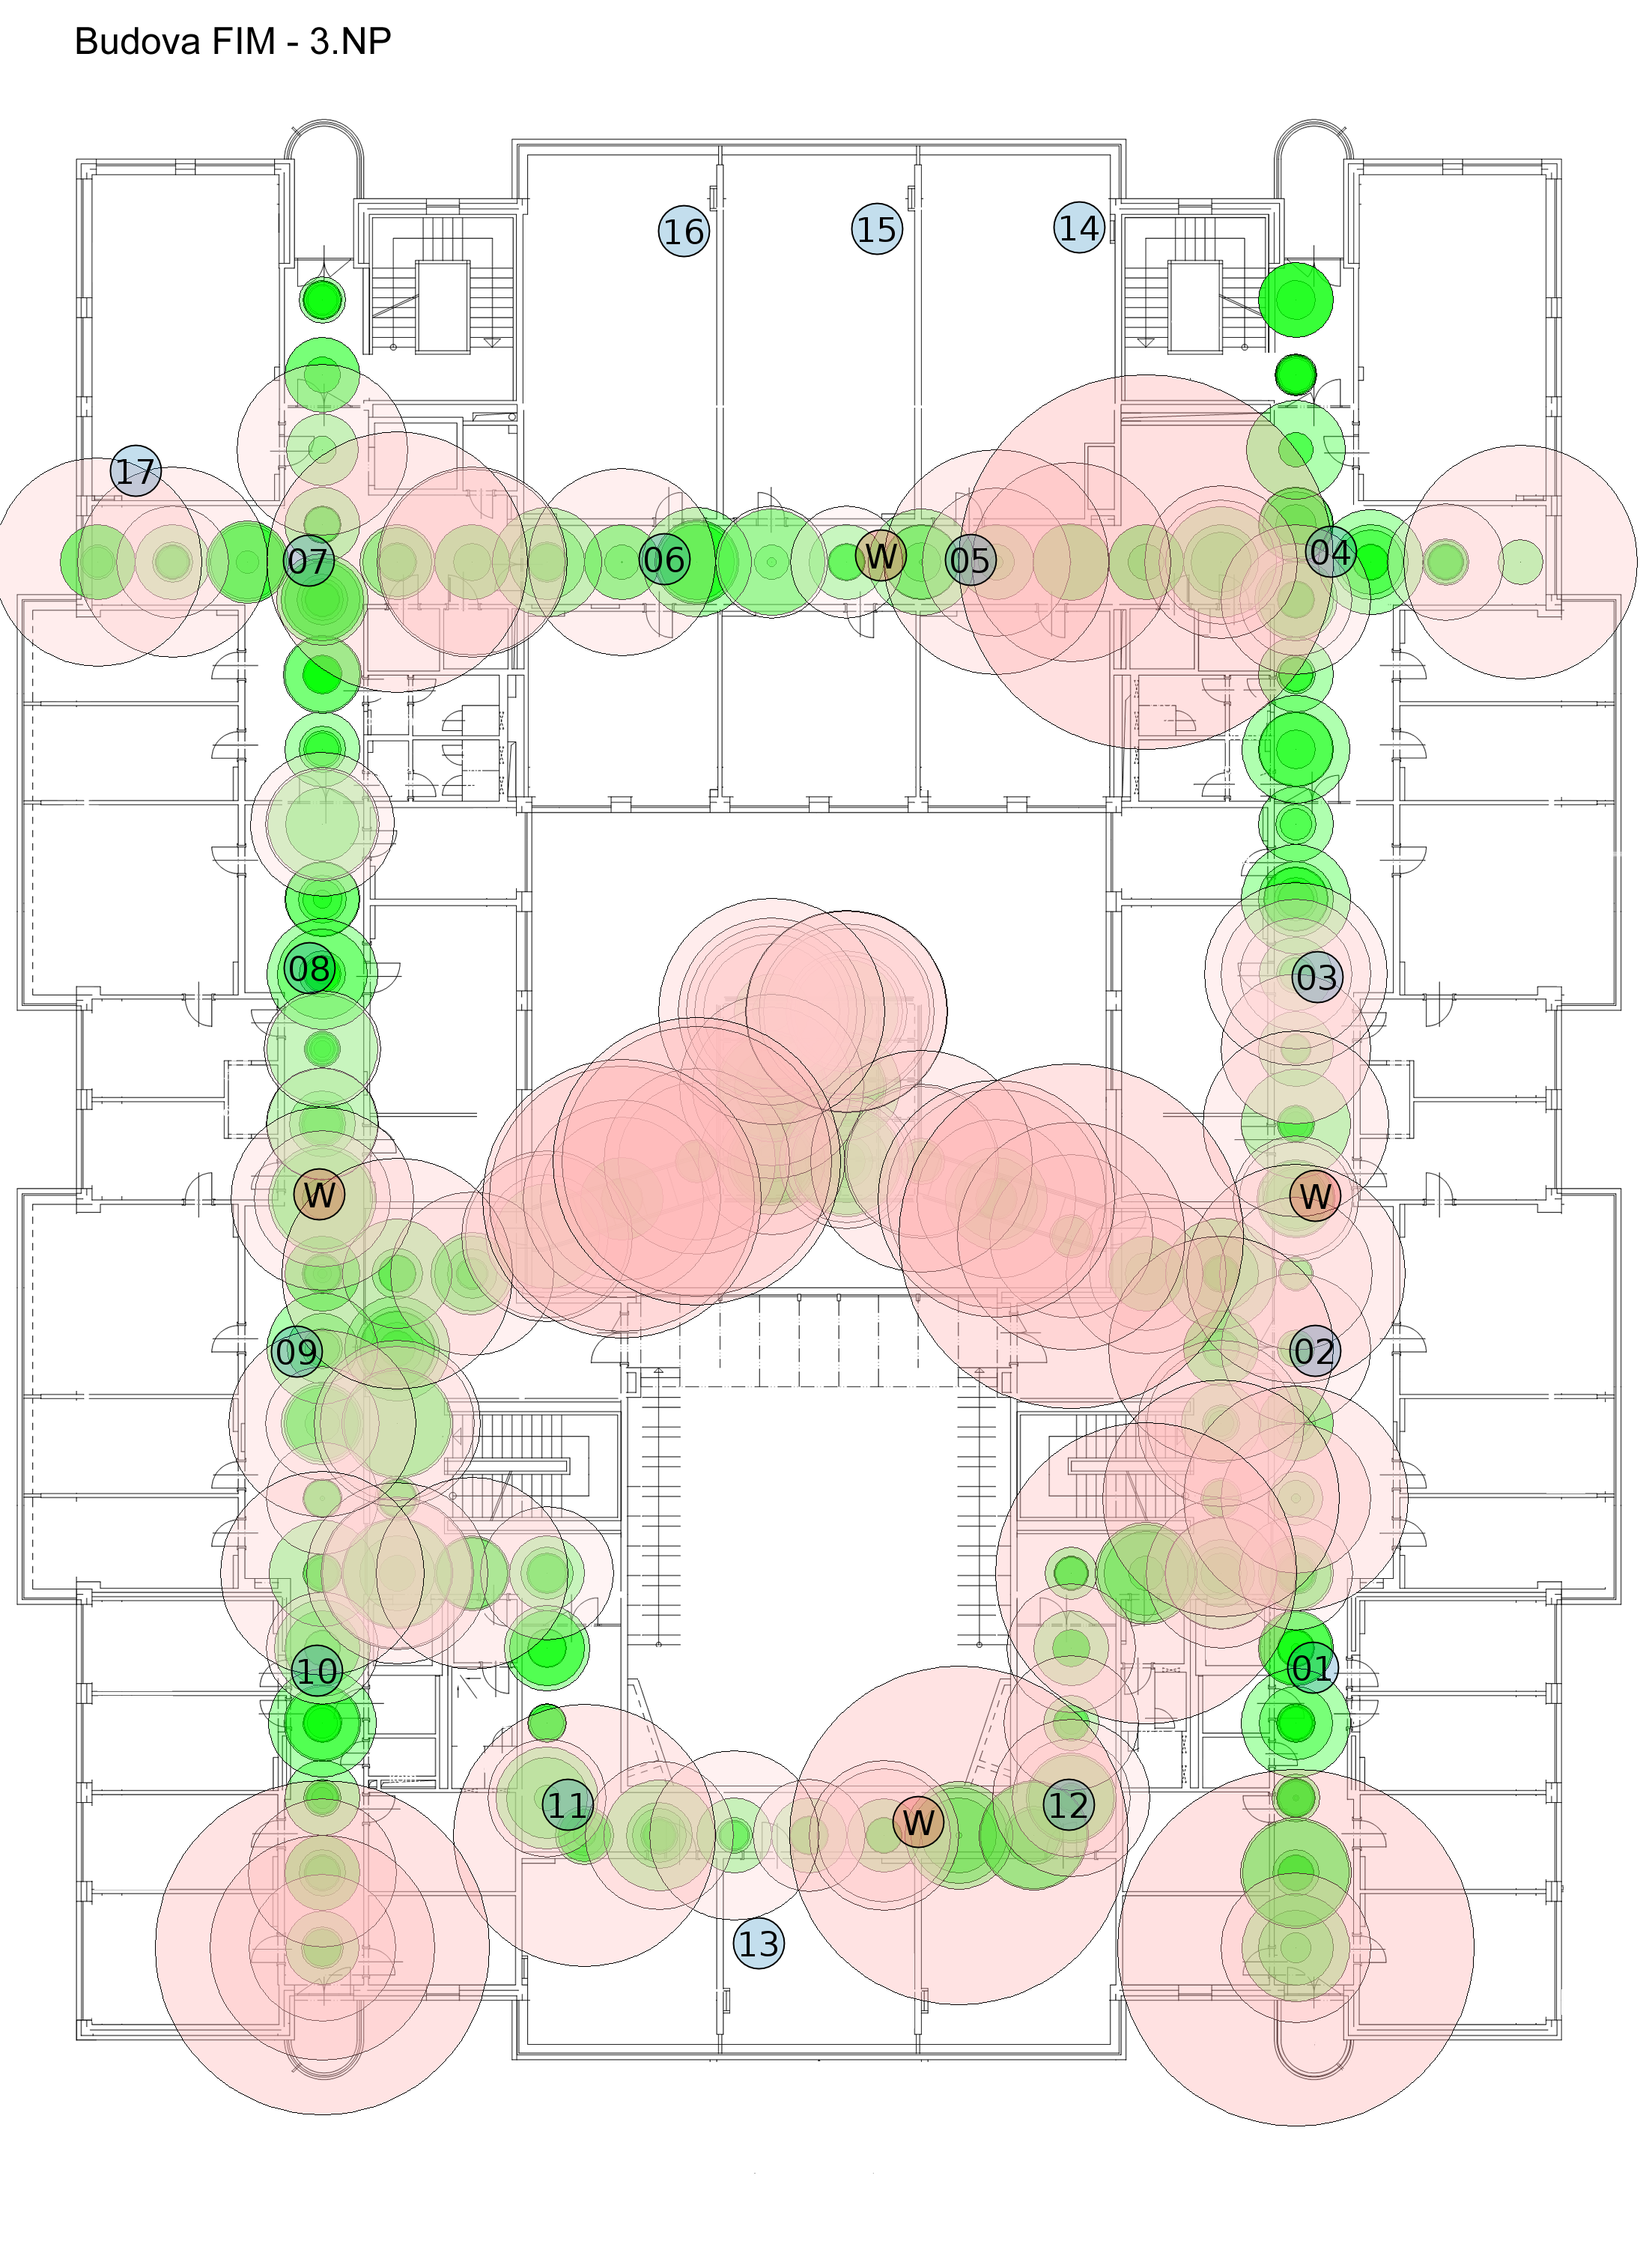
\includegraphics[width=0.38\textwidth]{img/combined_error_classic}
		\hspace{0.3cm}
		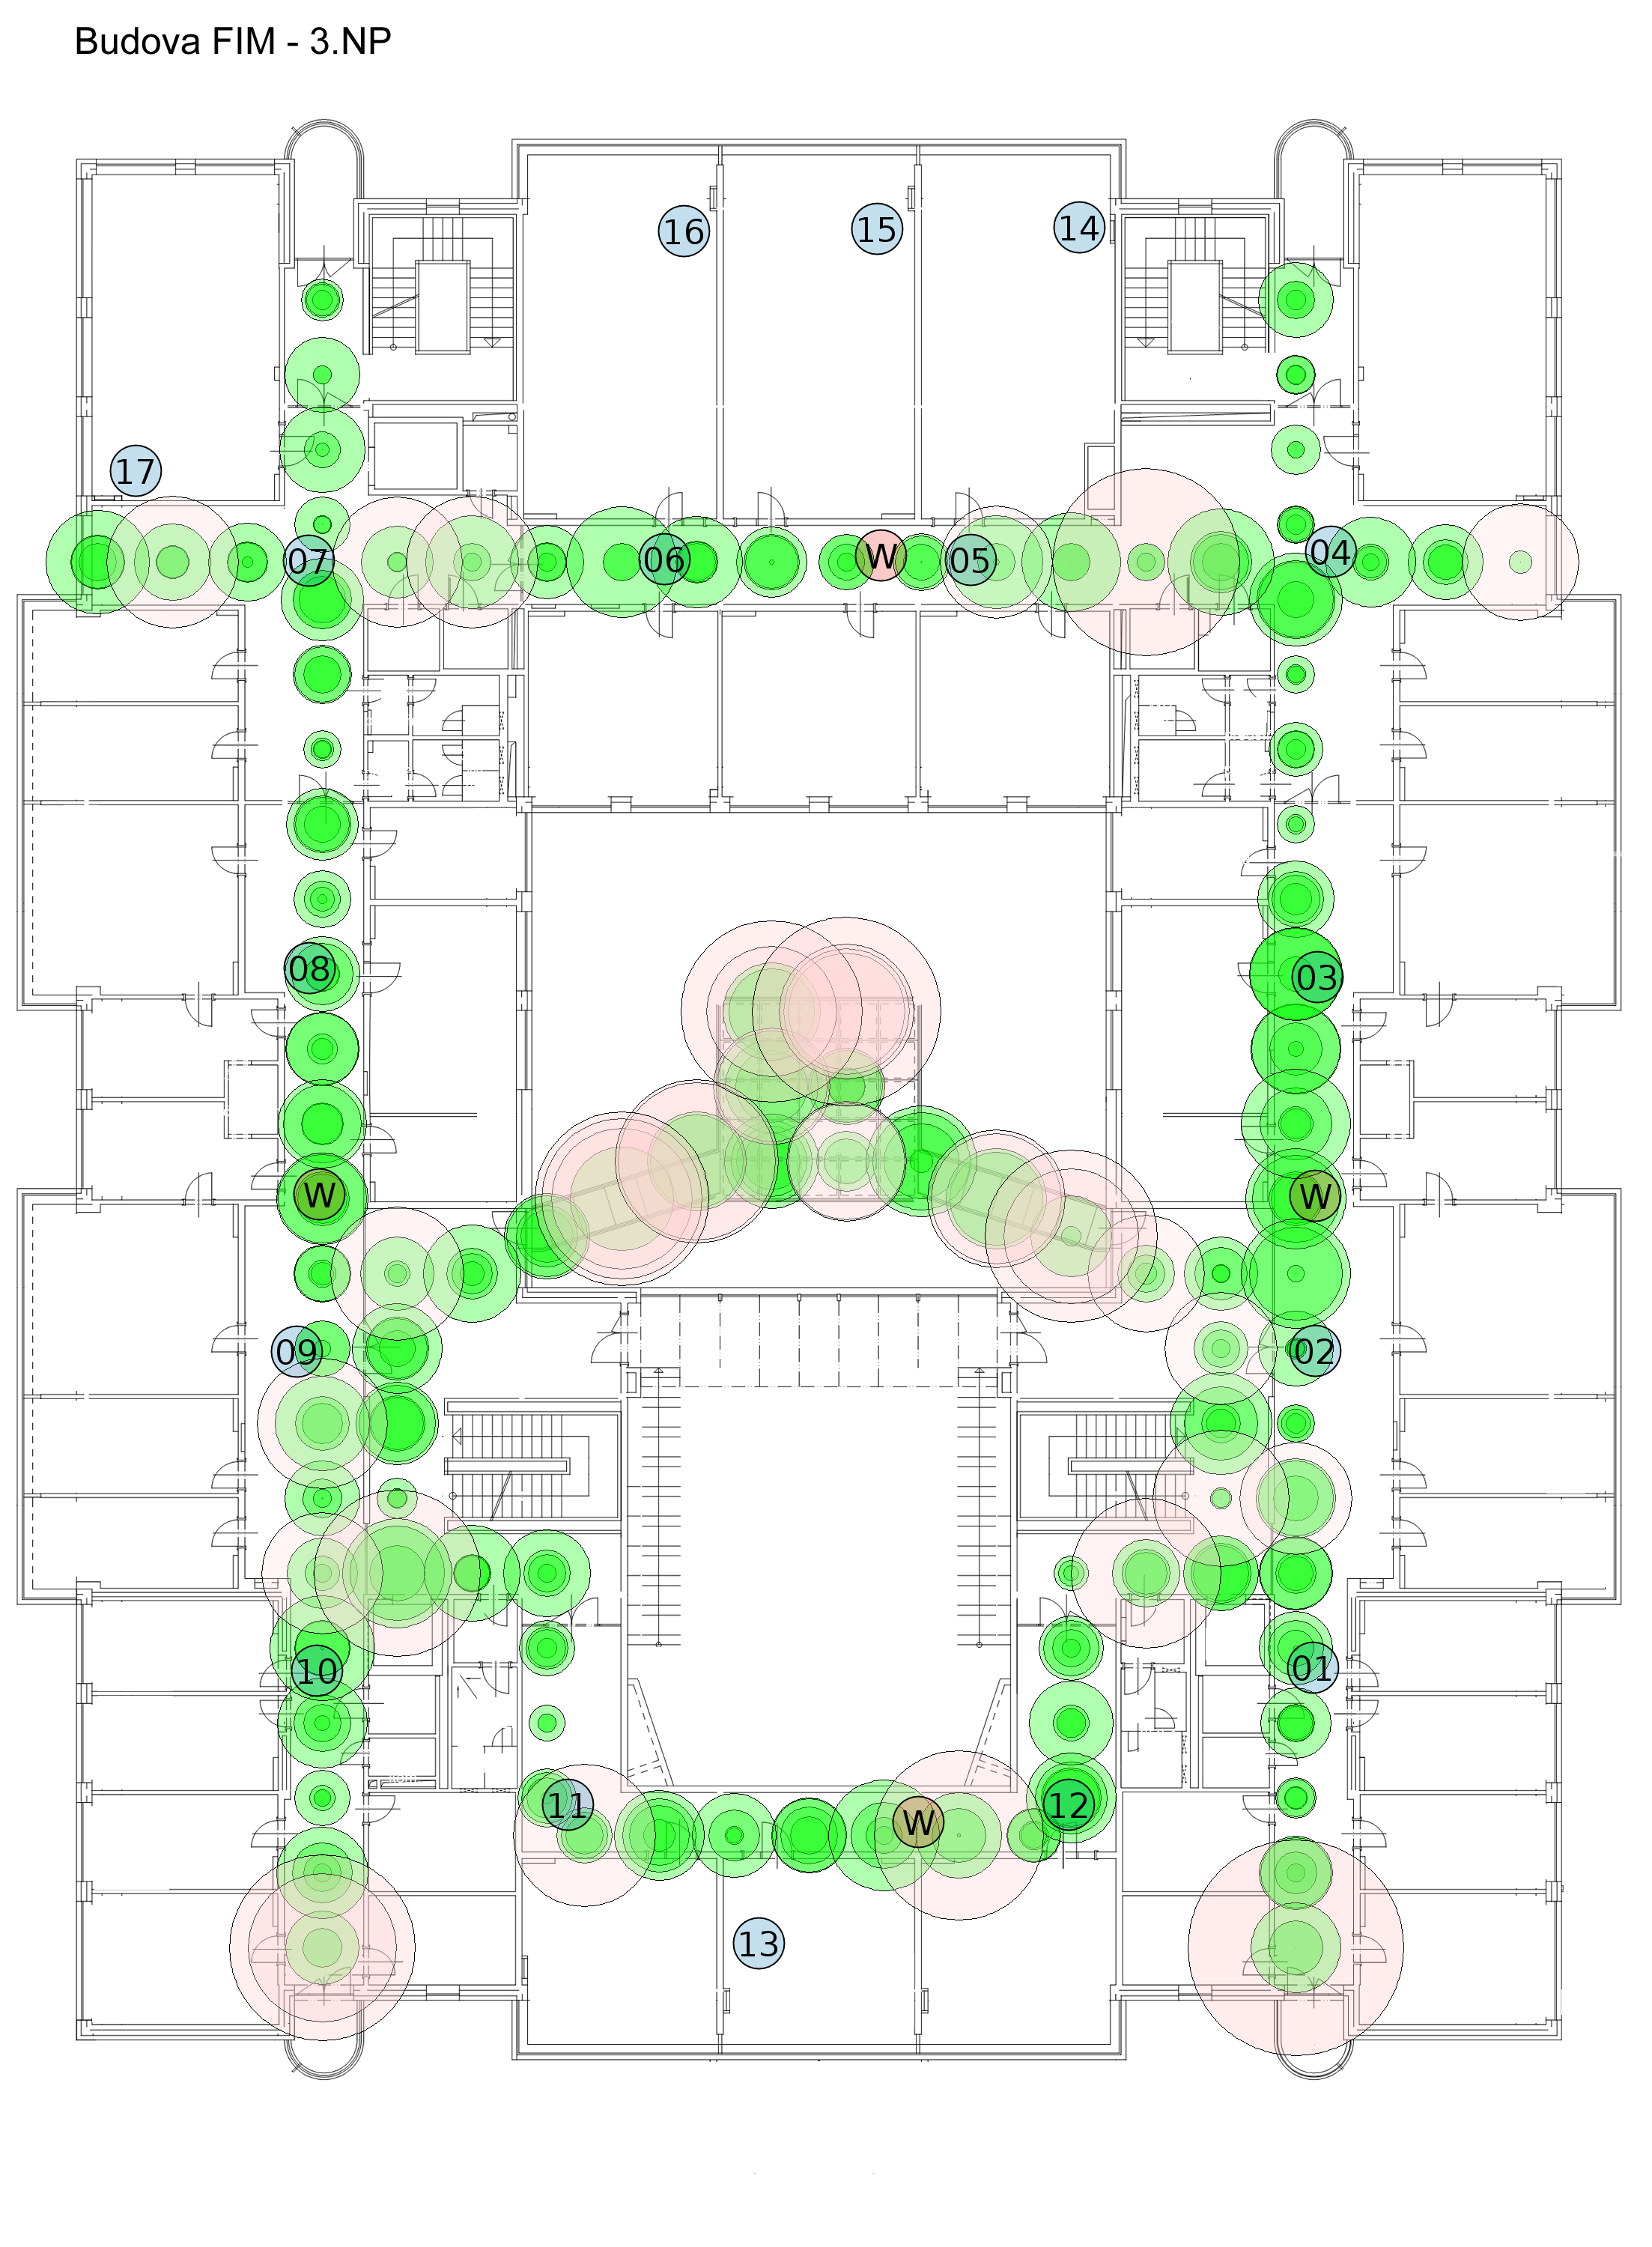
\includegraphics[width=0.38\textwidth]{img/combined_error_multiple_f}
		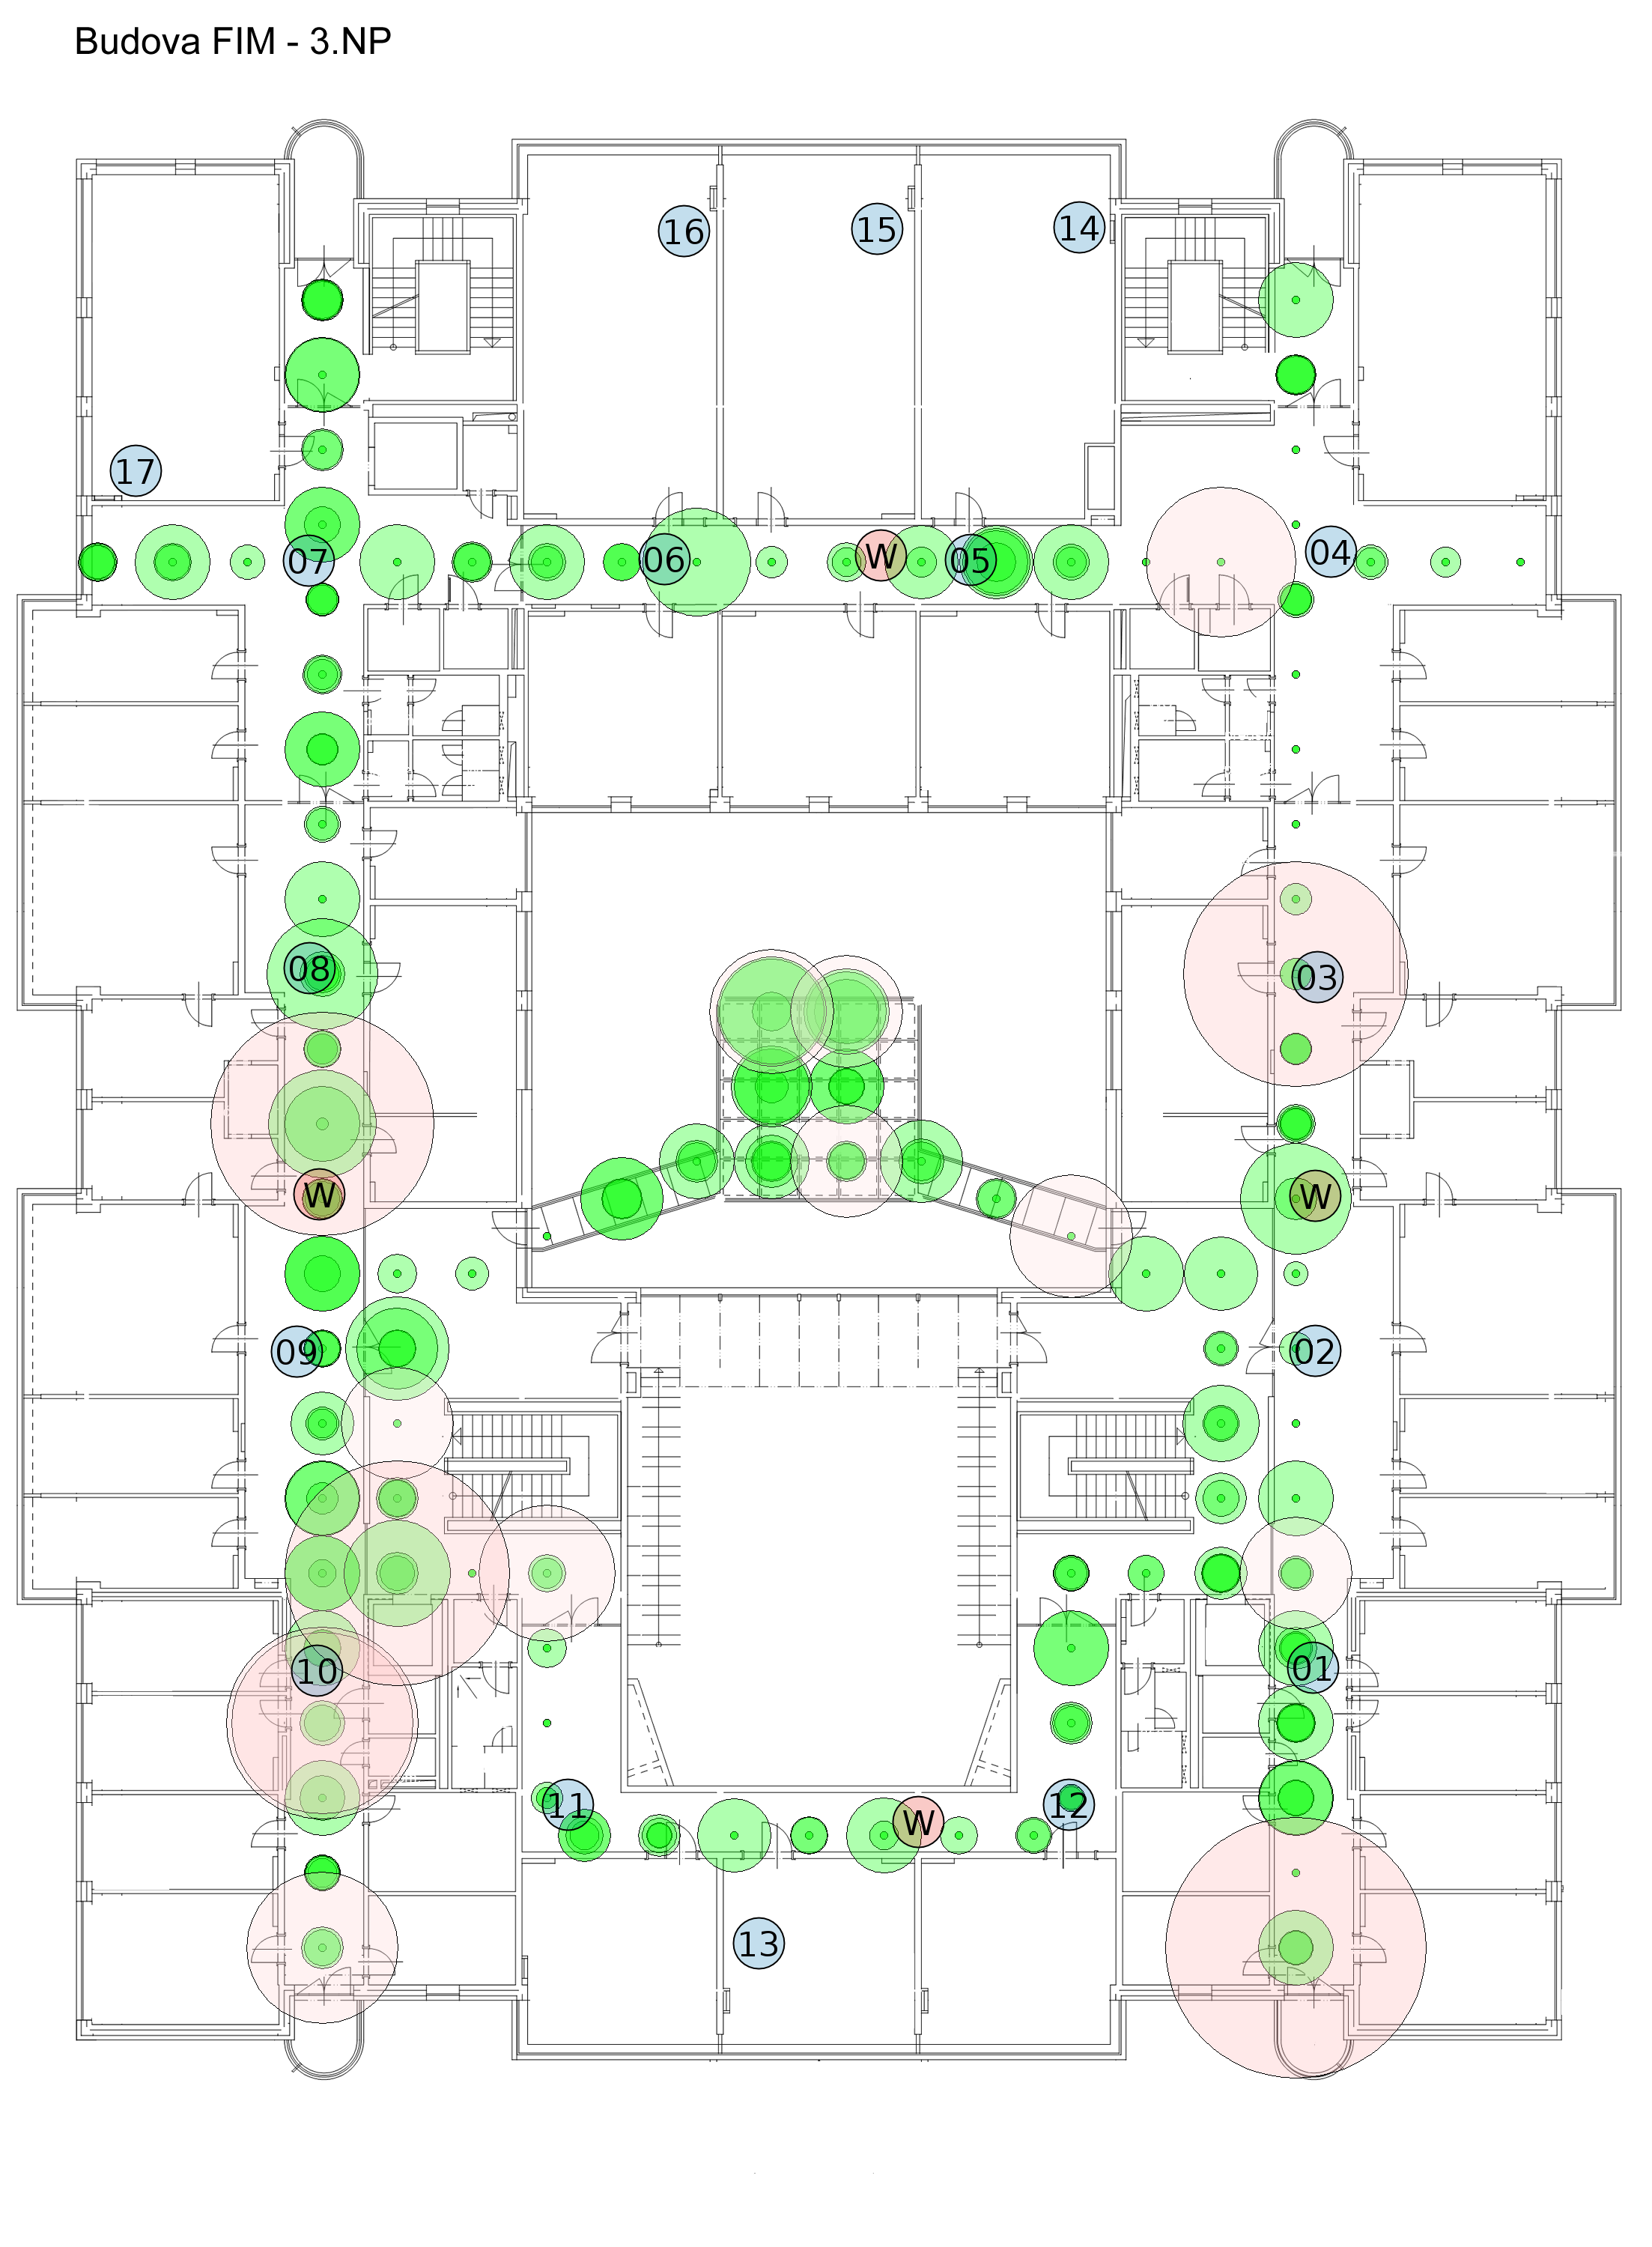
\includegraphics[width=0.38\textwidth]{img/combined_error_f_combination}
		\hspace{0.3cm}
		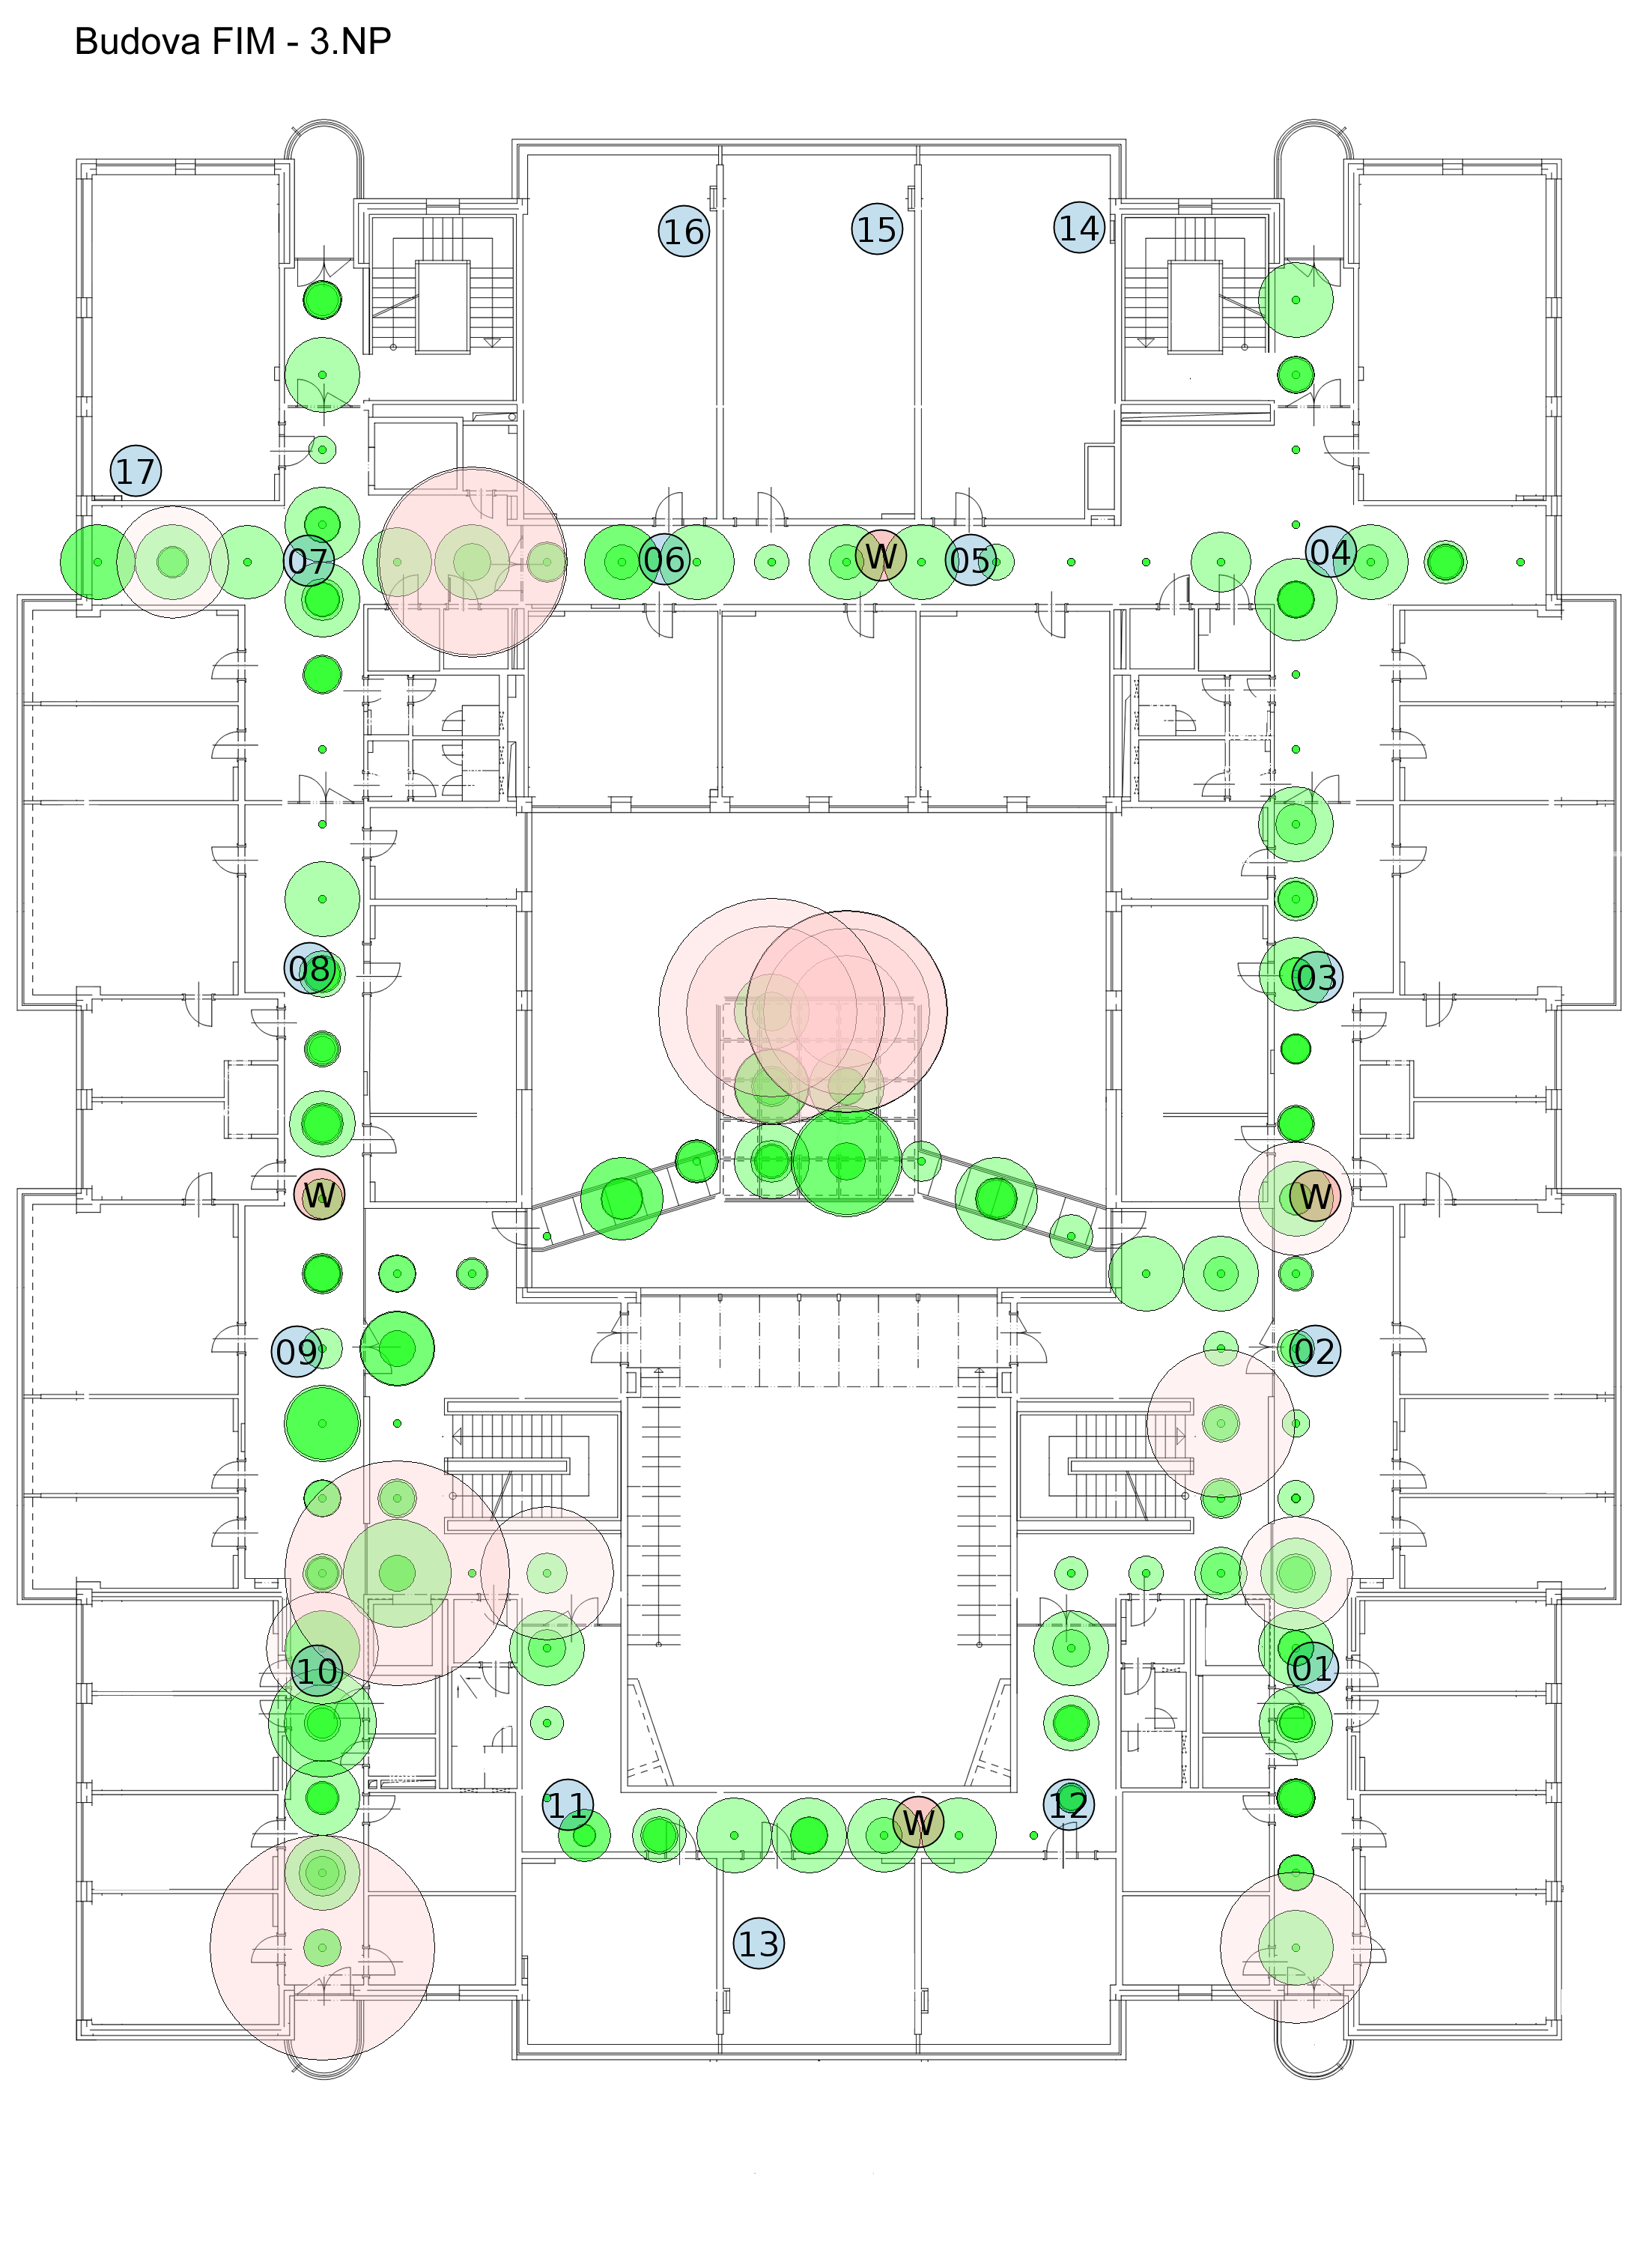
\includegraphics[width=0.38\textwidth]{img/phone_error}
		\par\end{centering}
	\caption{Maps of errors for all algorithms with last one for mobile error only}
	\label{fig09c06}
\end{figure}

\fref{fig09c06} shows map images for all previously described and evaluated algorithms with last one displaying mobile only evaluation. Top left image shows errors for classic evaluation that ignores device of origin. Top right is for the next round of evaluation which takes multiple fingerprints with different device origins, calculates their position and averages it to improve accuracy. Bottom left picture is for the last evaluation which combines multiple fingerprints into one. Finally, picture on the bottom right displays errors for mobile only localization used as a comparison with previous algorithms.  

Classic evaluation shows a big amount of orange circles, which means that error of a specific fingerprint is over three meters, and most of them seem to be in the middle of Campus building where there are no beacons placed associated with this floor. The other problematic spots seems to be in the south part of the building (bottom part of the map). Rest of the places are not considered as problematic since they usually have only one fingerprint with error over three meters. There are 119 fingerprints with error higher than three meters which is around 14\%.

Moving to the second image, it shows a big improvement of the localization for all positions and filtering out which places may actually be problematic. Bringing the count of fingerprints with error higher than three meters from 119 to 35, which is just 4\% of all fingerprints. And as for the final algorithm image (bottom left), it illustrates the best precision of all algorithms where 82 fingerprints have zero meters error and just 15 with error above three meters, bringing it down just under 2\%.